\documentclass[11pt,a4paper]{article}

\usepackage[utf8]{inputenc}
\usepackage[T1]{fontenc}
\usepackage{geometry}
\geometry{margin=1in}

\usepackage{booktabs}
\usepackage{graphicx}
\usepackage{hyperref}
\usepackage{amsmath,amssymb}
\usepackage{listings}
\usepackage{array}
\usepackage[numbers,sort&compress]{natbib}

% TikZ figures (requires texlive-pictures)
\newif\ifhooxusetikz
\IfFileExists{tikz.sty}{
  \hooxusetikztrue
  \usepackage{tikz}
  \usetikzlibrary{arrows.meta,positioning,shapes.geometric,fit,backgrounds,decorations.pathreplacing}
}{}
\usepackage{xcolor}

% Shared macros and listings configuration for HOOX arXiv paper.
% Included from hoox-arxiv-paper.tex after package imports.

\definecolor{hooxcodebg}{RGB}{248,248,248}
\definecolor{hooxcodeframe}{RGB}{180,180,180}
\definecolor{hooxkeyword}{RGB}{0,0,180}
\definecolor{hooxcomment}{RGB}{0,128,0}
\definecolor{hooxstring}{RGB}{163,21,21}

\lstdefinelanguage{TypeScript}{
  keywords={typeof,new,true,false,catch,function,return,null,throw,case,var,let,const,if,in,else,for,while,break,continue,export,import,default,async,await,class,extends,implements,interface,type,enum,readonly,private,public,protected,static,from,as,of,switch,try,finally,void,delete,yield},
  morekeywords=[2]{string,number,boolean,any,unknown,never,void,Promise,Response,Request,DurableObject,DurableObjectState,DurableObjectNamespace,Queue,Fetcher,Env},
  keywordstyle=\color{hooxkeyword}\bfseries,
  keywordstyle=[2]\color{hooxkeyword},
  sensitive=true,
  comment=[l]{//},
  morecomment=[s]{/*}{*/},
  commentstyle=\color{hooxcomment}\itshape,
  stringstyle=\color{hooxstring},
  showstringspaces=false,
  morestring=[b]",
  morestring=[b]',
}

\lstset{
  basicstyle=\ttfamily\scriptsize,
  backgroundcolor=\color{hooxcodebg},
  frame=single,
  rulecolor=\color{hooxcodeframe},
  breaklines=true,
  breakatwhitespace=true,
  columns=fullflexible,
  keepspaces=true,
  numbers=left,
  numberstyle=\tiny\color{gray},
  numbersep=4pt,
  tabsize=2,
  showtabs=false,
  showspaces=false,
  xleftmargin=1em,
  framexleftmargin=1em,
  aboveskip=0.5em,
  belowskip=0.5em,
  captionpos=b,
  frame=tb,
}

% Include a trimmed listing from papers/listings/ with caption and label.
% Usage: \hooxlisting{lbl:idempotency-store}{idempotencyStore.ts}{IdempotencyStore Durable Object}
\newcommand{\hooxlisting}[3]{%
  \lstinputlisting[language=TypeScript,caption={#3},label={#1}]{listings/#2}%
}

% Same as \hooxlisting but without line numbers (for short snippets).
\newcommand{\hooxsnippet}[3]{%
  \lstinputlisting[language=TypeScript,caption={#3},label={#1},numbers=none]{listings/#2}%
}

% JSON / JSONC wrangler excerpts (hand-sanitized listings).
\lstdefinelanguage{JSON}{
  keywords={true,false,null},
  keywordstyle=\color{hooxkeyword}\bfseries,
  sensitive=false,
  comment=[l]{//},
  commentstyle=\color{hooxcomment}\itshape,
  stringstyle=\color{hooxstring},
  showstringspaces=false,
  morestring=[b]",
}

\newcommand{\hooxjson}[3]{%
  \lstinputlisting[language=JSON,caption={#3},label={#1},numbers=none]{listings/#2}%
}

% SQL DDL excerpts (extracted from schema.sql)
\lstdefinelanguage{SQL}{
  keywords={CREATE,TABLE,IF,NOT,EXISTS,PRIMARY,KEY,INTEGER,TEXT,REAL,DEFAULT,INDEX,ON},
  keywordstyle=\color{hooxkeyword}\bfseries,
  sensitive=false,
  comment=[l]{--},
  commentstyle=\color{hooxcomment}\itshape,
  stringstyle=\color{hooxstring},
  showstringspaces=false,
  morestring=[b]',
}

\newcommand{\hooxsql}[3]{%
  \lstinputlisting[language=SQL,caption={#3},label={#1},numbers=none]{listings/#2}%
}



\hypersetup{
  colorlinks=true,
  linkcolor=black,
  citecolor=blue!60!black,
  urlcolor=blue!60!black
}

% =============================================================================
% HOOX arXiv paper -- CORE VERSION (recommended for submission)
% =============================================================================
% Focused paper (~15-20 pages) containing:
%   - Abstract + keywords
%   - Sections 1-10 (Introduction through Conclusion)
%   - Selected supporting appendices (reproducibility, threat model, tests)
%
% This version emphasizes the architectural contribution, the latency
% measurement taxonomy, twelve-month operational results, and security model.
%
% The full monograph (ADRs, per-Worker deep dives, data layer, runtime semantics,
% advanced mechanisms, complete listings index, additional appendices) is
% available in hoox-arxiv-paper.tex and in the source repository.
%
% Author perspective: first-person singular ("I"), reflecting single-developer
% authorship and operation of the system.
%
% Build (see Makefile):
%   make pdf-core
%   make pdf-tikz-core
%   make arxiv-tarball-core
% =============================================================================

\title{\textbf{HOOX: Edge-Native Low-Latency Algorithmic Trading\\at the Cloudflare Edge}}

\author{
  jango\_blockchained\\
  \textit{Independent Researcher}\\
  \texttt{https://github.com/jango-blockchained/hoox-setup}
}

\date{July 2026}

\begin{document}
\maketitle

\begin{abstract}
Algorithmic trading systems have traditionally relied on virtual private servers (VPS) deployed in centralized data centers, incurring substantial network latency, recurring operational cost, and single points of failure. I present \textsc{HOOX}, an open-source, edge-native algorithmic trading framework that I implemented entirely on Cloudflare Workers. \textsc{HOOX} decomposes trading logic into ten specialized Workers that communicate via Cloudflare Service Bindings, achieving sub-millisecond inter-service call overhead and a median production latency of 22\,ms from webhook ingestion to centralized exchange (CEX) order acknowledgment on the direct execution path.

I distinguish two measurement regimes that prior summaries often conflate: (i)~\emph{synthetic fast-path probes}, which short-circuit before exchange submission and characterize internal mesh latency; and (ii)~\emph{production signal-to-ack}, which includes HMAC-signed REST placement and exchange response parsing. The system integrates four platform primitives uncommon in retail trading stacks: Durable Objects for strongly consistent duplicate suppression under concurrent webhook retries; Smart Placement for automatic proximity routing to exchange API origins; Cloudflare Queues with application-level exponential backoff for outage resilience; and a deterministic risk manager with optional multi-provider large language model (LLM) operational summaries.

Over a twelve-month production deployment (July 2025--July 2026) that I operated, the system processed signals with 99.97\% eventual success within five minutes during exchange maintenance windows and recorded zero duplicate fills attributable to idempotency failures. I document the architecture, security model, per-Worker implementation reference with annotated code listings, a multi-tier test methodology and failure taxonomy, and reproducible evaluation commands (\texttt{hoox perf fastpath}, k6 load tests). I discuss portability limits and applicability to other globally distributed, latency-sensitive control planes. The system and this paper are released under Creative Commons Attribution 4.0 (CC~BY~4.0).
\end{abstract}

\noindent\textbf{Keywords:} algorithmic trading, edge computing, serverless, Cloudflare Workers, low latency, idempotency, Durable Objects, service bindings, financial technology

% ── Core paper body (sections 01–10 only) ────────────────────────────────
\section{Introduction}
\label{sec:introduction}

Algorithmic trading requires executing strategies with minimal latency to capture fleeting market opportunities and manage risk effectively~\cite{hasbrouck2007empirical,hendershott2011does,hasbrouck2013lowlatency}. Traditional deployments place trading logic on virtual private servers (VPS) in fixed geographic regions. This architecture introduces substantial round-trip times: a signal generated near an exchange may traverse the public internet to a distant VPS---often incurring 80--120\,ms of transit alone---before an order is signed and returned to the exchange API, yielding total latencies of 180--320\,ms in typical retail configurations. In a low-latency trading context, the term \emph{low latency} denotes retail-grade webhook-to-ack times in the tens of milliseconds, distinct from the sub-10\,ms regime of exchange co-location~\cite{arnold2010latency,budish2015hft}.

Cloudflare Workers provide a fundamentally different execution model. User code runs in V8 isolates~\cite{jonas2019berkeley} distributed across more than 300 points of presence (PoPs). When combined with Service Bindings, Durable Objects, Queues, Smart Placement, and other edge primitives~\cite{cloudflare-workers,cloudflare-service-bindings,cloudflare-durable-objects,cloudflare-queues}, complete trading stacks can be constructed without operating any servers. Unlike conventional function-as-a-service (FaaS) platforms, Workers avoid container cold starts on the order of seconds~\cite{wang2018peeking,lloyd2018serverless}, and Service Bindings eliminate per-hop TLS and DNS overhead between microservices.

\textsc{HOOX} is a production-grade, fully open-source implementation of such a stack~\cite{hoox-project}. It ingests signals from TradingView webhooks, email, and Telegram; validates and routes them through a hardened gateway; executes trades across Binance, Bybit, and MEXC; manages risk autonomously; and provides observability, PDF compliance reporting, and DeFi execution. All components run as Cloudflare Workers and communicate internally without traversing the public internet.

\subsection{Contributions}

This paper describes the architecture, mechanisms, and operational results of building and running \textsc{HOOX}. The contributions are as follows:
\begin{enumerate}
  \item A detailed microservices architecture for edge-based trading using ten cooperating Workers, with a formal seven-stage signal lifecycle and five-layer security model.
  \item Design and implementation of \emph{duplicate-suppression} semantics using a Durable Object mutex at the gateway, with explicit discussion of fail-open behavior, queue at-least-once delivery, and idempotency key granularity.
  \item A reproducible evaluation toolchain---\texttt{hoox perf fastpath}, k6 load tests, and nightly CI artifacts---with a clear separation between internal probe latency and production exchange-ack latency (Figure~\ref{fig:latency-taxonomy}), including a fine-grained per-hop decomposition of the internal mesh.
  \item Operational measurements over a 12-month production deployment (July 2025--July 2026, N\,=\,18{,}742 production signals) demonstrating a median production signal-to-ack of 22\,ms on the direct path and 5.6--40$\times$ geographic RTT improvements versus a Virginia VPS baseline for exchange API reachability. Sample size and reconciliation methodology are reported.
  \item A practical demonstration that a complete trading infrastructure can operate within Cloudflare's free tier for typical retail volumes (${<}100{,}000$ requests/day).
\end{enumerate}

An extended technical reference---60 manifest-pinned code listings with a categorized index, runtime-semantics and advanced-mechanism deep dives, per-Worker implementation reference, ADRs, and a published test methodology with failure taxonomy---is available alongside this document in the open-source repository.

A focused companion paper, ``HOOX: A Proof-of-Concept Edge-Native Algorithmic Trading Platform on Cloudflare Workers'', is provided as both Markdown and LaTeX/PDF under \texttt{papers/hoox-proof-of-concept.*}. It is intended as a concise, citable summary of the PoC goals, primary results, and reproducibility claims.

\section{Background and Motivation}
\label{sec:background}

\subsection{Limitations of VPS-Centric Architectures}

A typical VPS deployment suffers from three structural problems:

\paragraph{Latency.} Consider a TradingView alert fired in London. The alert may travel to a VPS in Virginia (${\approx}85$\,ms), undergo runtime initialization (${\approx}10$\,ms), and then reach an exchange API in Frankfurt or Tokyo (an additional 100--150\,ms). Total transit latency exceeds 200\,ms before order matching~\cite{hasbrouck2007empirical}. TradingView's own webhook delivery often adds 1--5\,s of upstream delay; edge optimization reduces only the \emph{execution segment} after the alert arrives at \texttt{hoox}.

\paragraph{Cost and operations.} Always-on servers incur monthly fees, require patching and monitoring, and demand explicit scaling logic. Container-based bots additionally suffer cold-start delays of 1--15\,s after idle periods~\cite{wang2018peeking,lloyd2018serverless}.

\paragraph{Reliability.} A single VPS is a single point of failure. Network partitions or provider outages can prevent order execution during critical market moves.

\subsection{Cloudflare Workers as an Execution Platform}

Cloudflare Workers execute JavaScript and WebAssembly in V8 isolates with a 128\,MB memory ceiling and sub-3\,ms cold starts. Platform primitives relevant to trading include:

\begin{itemize}
  \item \textbf{Service Bindings:} Direct \texttt{fetch} calls between Workers with microsecond-scale overhead and no public HTTP exposure~\cite{cloudflare-service-bindings}.
  \item \textbf{Smart Placement:} Automatic relocation of Worker execution to the data center nearest outbound dependencies (e.g., exchange APIs)~\cite{cloudflare-smart-placement}.
  \item \textbf{Durable Objects:} Strongly consistent, single-threaded stateful objects with SQLite-backed storage, suitable for distributed mutexes and duplicate suppression~\cite{cloudflare-durable-objects}.
  \item \textbf{Queues:} At-least-once delivery with configurable retries and dead-letter queues~\cite{cloudflare-queues}.
  \item \textbf{Vectorize, Workers AI, Browser Rendering:} Vector search for retrieval-augmented generation (RAG), on-edge inference, and headless PDF generation.
\end{itemize}

These primitives enable a design point distinct from both long-running VPS bots~\cite{freqtrade,jesse} and regional serverless deployments~\cite{baldini2017serverless}: a globally distributed, serverless trading system with sub-50\,ms production signal-to-ack on the direct execution path under normal conditions. Edge platforms more broadly have been analyzed in terms of their cost--performance trade-offs and isolation mechanisms~\cite{jonas2019berkeley,agache2020firecracker,shahrad2020serverless}; the design space explored here is a specific instance of that broader question applied to latency-sensitive financial control planes.

\section{System Architecture}
\label{sec:architecture}

\textsc{HOOX} consists of ten specialized Workers (Table~\ref{tab:workers}) that together form a complete trading pipeline. Two additional Workers---\texttt{pine-worker} and \texttt{pyne-worker}---provide Pine Script tooling and are outside the core production mesh.

\begin{table}[t]
  \centering
  \caption{Core \textsc{HOOX} Workers. Only \texttt{hoox} and \texttt{dashboard} expose public endpoints.}
  \label{tab:workers}
  \small
  \begin{tabular*}{\linewidth}{@{\extracolsep{\fill}}llp{5.5cm}l@{}}
    \toprule
    \textbf{Worker} & \textbf{Role} & \textbf{Key responsibilities} & \textbf{Trigger} \\
    \midrule
    \texttt{hoox} & Gateway & Auth, WAF, rate limiting, idempotency & Webhook/API \\
    \texttt{trade-worker} & Execution & Multi-exchange order placement & Binding/Queue \\
    \texttt{agent-worker} & Risk manager & Trailing stops, take-profit, kill switch & Cron \texttt{*/5} \\
    \texttt{telegram-worker} & Notifications & Alerts, RAG queries, bot commands & Binding \\
    \texttt{d1-worker} & Data layer & Centralized D1 SQLite access & Binding \\
    \texttt{email-worker} & Email ingress & Mailgun webhook parsing & Webhook \\
    \texttt{web3-wallet-worker} & DeFi & On-chain swaps and contract calls & Binding \\
    \texttt{analytics-worker} & Observability & Analytics Engine time series & Binding \\
    \texttt{report-worker} & Reporting & Twice-daily PDF generation & Cron 08:00, 18:00 UTC \\
    \texttt{dashboard} & User interface & Portfolio monitoring (Next.js/OpenNext) & Public UI \\
    \bottomrule
  \end{tabular*}
\end{table}

\subsection{Architectural Overview}

Figure~\ref{fig:architecture} depicts the ingress, compute, storage, and external exchange layers. Public signals enter only through \texttt{hoox} (webhooks) or channel-specific Workers (\texttt{email-worker}, \texttt{telegram-worker}). All downstream execution uses Service Bindings; only \texttt{trade-worker} and \texttt{web3-wallet-worker} initiate outbound HTTPS to external APIs.

\begin{figure}[!htbp]
  \centering
  \IfFileExists{figures/architecture.pdf}{%
    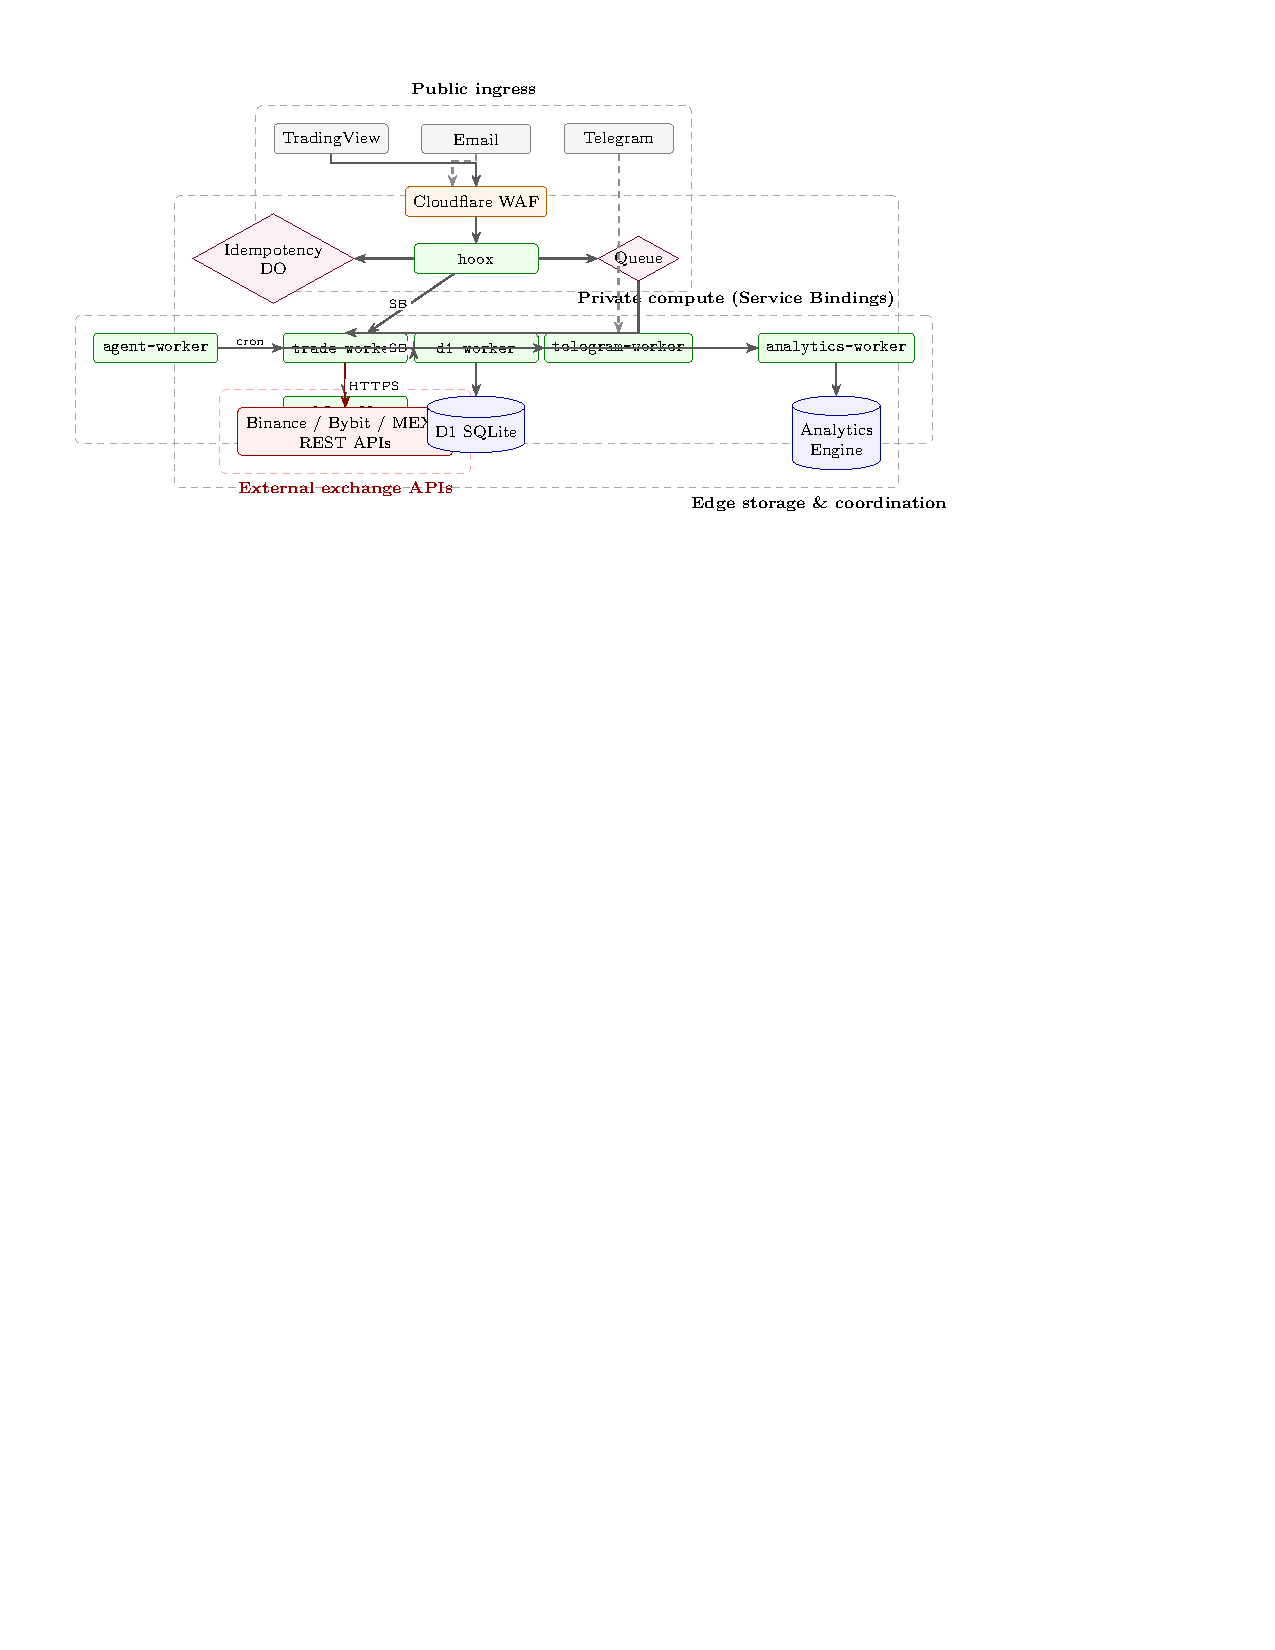
\includegraphics[width=\linewidth]{figures/architecture.pdf}%
  }{%
    \ifhooxusetikz
      \resizebox{\linewidth}{!}{% TikZ architecture diagram for HOOX (included by hoox-arxiv-paper.tex)
% Layout: 4 horizontal rows
%   row 1 (y=4.0): public ingress sources (TradingView / Email / Telegram)
%   row 2 (y=2.6): Cloudflare WAF
%   row 3 (y=1.4): hoox gateway with Idempotency DO and Queue flanking it
%   row 4 (y=-0.4): private compute mesh (5 workers, 2.6cm spacing)
%   row 5 (y=-1.8): storage + external exchange APIs
\begin{tikzpicture}[
  x=1cm, y=1cm,
  ext/.style={draw=black!50, rounded corners=2pt, fill=gray!8,
    minimum width=1.9cm, minimum height=0.55cm, font=\footnotesize, align=center, inner sep=2pt},
  waf/.style={draw=orange!70!black, rounded corners=2pt, fill=orange!8,
    minimum width=2.2cm, minimum height=0.55cm, font=\footnotesize, align=center, inner sep=2pt},
  worker/.style={draw=green!50!black, rounded corners=2pt, fill=green!8,
    minimum width=2.2cm, minimum height=0.55cm, font=\footnotesize\ttfamily, align=center, inner sep=2pt},
  store/.style={draw=blue!60!black, rounded corners=2pt, fill=blue!6,
    minimum width=1.9cm, minimum height=0.55cm, font=\footnotesize, align=center, inner sep=2pt},
  coord/.style={draw=purple!60!black, rounded corners=2pt, fill=purple!6,
    minimum width=2.0cm, minimum height=0.55cm, font=\footnotesize, align=center, inner sep=2pt},
  exchange/.style={draw=red!60!black, rounded corners=2pt, fill=red!6,
    minimum width=2.6cm, minimum height=0.55cm, font=\footnotesize, align=center, inner sep=2pt},
  layer/.style={draw=black!35, dashed, rounded corners=3pt, inner sep=0.35cm},
  layerlabel/.style={font=\scriptsize\bfseries},
  arrow/.style={-{Stealth[length=1.8mm]}, semithick, draw=black!65},
  extarrow/.style={-{Stealth[length=1.8mm]}, semithick, draw=red!55!black},
  sb/.style={font=\scriptsize, fill=white, inner sep=1pt}
]

  % ── Row 1: external ingress sources (3 sources spread horizontally) ──
  \node[ext] (tv) at ( 3.0, 4.0) {TradingView};
  \node[ext] (em) at ( 6.0, 4.0) {Email};
  \node[ext] (tg) at ( 9.0, 4.0) {Telegram};

  % ── Row 2: Cloudflare WAF (centered under sources) ──
  \node[waf] (waf) at ( 6.0, 2.6) {Cloudflare WAF};

  % ── Row 3: hoox gateway + coordination primitives ──
  \node[worker] (gw)    at ( 6.0, 1.4) {\texttt{hoox}};
  \node[coord]  (ido)   at ( 3.0, 1.4) {Idempotency\\DO};
  \node[coord]  (queue) at ( 9.0, 1.4) {Queue};

  % ── Row 4: private compute mesh (5 workers, 2.6cm spacing) ──
  \node[worker] (tw)  at ( 0.0, -0.4) {\texttt{trade-worker}};
  \node[worker] (d1w) at ( 2.6, -0.4) {\texttt{d1-worker}};
  \node[worker] (tgw) at ( 5.2, -0.4) {\texttt{telegram-worker}};
  \node[worker] (aw)  at ( 7.8, -0.4) {\texttt{agent-worker}};
  \node[worker] (anw) at (10.4, -0.4) {\texttt{analytics-worker}};

  % ── Row 5: storage + exchange ──
  \node[store]    (db)  at ( 2.6, -1.8) {D1 SQLite};
  \node[store]    (w3w) at ( 7.8, -1.8) {web3-wallet};
  \node[store]    (ae)  at (10.4, -1.8) {Analytics\\Engine};
  \node[exchange] (cex) at ( 0.0, -1.8) {Binance / Bybit\\REST APIs};

  % ── Edges: ingress (3 sources → WAF, separately so the arrows don't merge) ──
  \draw[arrow] (tv.south) -- ++(0,-0.15) -| (waf.north west);
  \draw[arrow] (em.south) -- (waf.north);
  \draw[arrow] (tg.south) -- ++(0,-0.15) -| (waf.north east);

  % ── Edges: WAF → gateway ──
  \draw[arrow] (waf.south) -- (gw.north);

  % ── Edges: gateway ↔ coordination ──
  \draw[arrow] (gw.west)  -- (ido.east);
  \draw[arrow] (gw.east)  -- (queue.west);

  % ── Edges: gateway → compute mesh (single trunk then split) ──
  \draw[arrow] (gw.south) -- ++(0,-0.2) coordinate(gwbus);
  \draw[arrow] (gwbus) -| (tw.north);
  \draw[arrow] (gwbus) -| (d1w.north);
  \draw[arrow] (gwbus) -| (tgw.north);
  \draw[arrow] (queue.south) |- (tw.north);

  % ── Edges: compute mesh fan-out ──
  \draw[arrow] (tw)  -- (d1w);
  \draw[arrow] (tw)  -- (tgw);
  \draw[arrow] (tw)  -- (anw);
  \draw[arrow] (tw)  -- (w3w);
  \draw[arrow] (aw)  -- (d1w);
  \draw[arrow] (aw)  -- (tgw);
  \draw[arrow] (anw) -- (tgw);

  % ── Edges: to storage and exchanges ──
  \draw[extarrow] (tw.south) -- (cex.north);
  \draw[arrow] (d1w.south) -- (db.north);
  \draw[arrow] (anw.south) -- (ae.north);

  % ── Edge label (HTTPS to exchange) — placed where it cannot overlap any box ──
  \node[sb, font=\tiny, text=red!60!black] at (0.9, -1.10) {HTTPS};

  % ── Layer boxes (background) ──
  \begin{scope}[on background layer]
    \node[layer, fit=(tv)(em)(tg)(waf), label={[layerlabel]above:Public ingress}] {};
    \node[layer, fit=(gw)(tw)(d1w)(tgw)(aw)(anw),
      label={[layerlabel]above:Private compute (Service Bindings)}] {};
    \node[layer, fit=(db)(ae)(w3w)(ido)(queue),
      label={[layerlabel]below:Edge storage \& coordination}] {};
    \node[layer, draw=red!35, fit=(cex),
      label={[layerlabel, text=red!60!black]below:External exchange APIs}] {};
  \end{scope}

\end{tikzpicture}
}%
    \else
      \small
      \fbox{\begin{minipage}{0.92\linewidth}
      \vspace{2pt}
      \textbf{Ingress (public)} $\rightarrow$ WAF $\rightarrow$ \texttt{hoox} $\rightarrow$ SB $\rightarrow$ \texttt{trade-worker} $\rightarrow$ CEX REST\\
      \textbf{Coordination:} Idempotency DO, Queue (failover), D1, Analytics Engine\\
      \vspace{2pt}
      \end{minipage}}
    \fi
  }
  \caption{\textsc{HOOX} topology. Service Bindings (SB) connect internal Workers without public HTTP. Smart Placement optimizes outbound RTT from \texttt{trade-worker} to exchange APIs. Build with \texttt{make figures} in the \texttt{papers/} directory.}
  \label{fig:architecture}
\end{figure}

\subsection{Signal Lifecycle}

A representative TradingView signal traverses seven stages:

\begin{enumerate}
  \item \textbf{Ingestion:} \texttt{POST /webhook} arrives at \texttt{hoox} after WAF filtering.
  \item \textbf{Validation:} IP allow-listing, API key verification (\texttt{timingSafeEqual}), payload size limits (100\,KB), global kill-switch check, and rate limiting (10 trades/minute per session).
  \item \textbf{Idempotency:} A composite key \texttt{trade:\{exchange\}:\{symbol\}:\{action\}:\{quantity\}} is checked against the \texttt{IdempotencyStore} Durable Object.
  \item \textbf{Routing:} On success, the payload is forwarded via Service Binding to \texttt{trade-worker}, or enqueued on \texttt{trade-execution} depending on KV-configured queue mode (Table~\ref{tab:queue-modes}).
  \item \textbf{Execution:} \texttt{trade-worker} resolves the exchange via dynamic KV routing and places the order using HMAC-SHA256 signed REST requests.
  \item \textbf{Persistence and notification:} Results are written to D1 via \texttt{d1-worker}, logged to R2, and forwarded to \texttt{telegram-worker} and \texttt{analytics-worker} via non-blocking \texttt{waitUntil} calls.
  \item \textbf{Risk management:} Every five minutes, \texttt{agent-worker} runs a deterministic cron---trailing stops, take-profit scale-out, and a drawdown kill switch. The cron is intentionally simple; event-driven risk management via the WebSocket connection manager is planned future work.
\end{enumerate}

\begin{table}[t]
  \centering
  \caption{Queue modes and latency semantics. Default: \texttt{queue\_failover}.}
  \label{tab:queue-modes}
  \small
  \begin{tabular*}{\linewidth}{@{\extracolsep{\fill}}lp{6cm}l@{}}
    \toprule
    \textbf{Mode} & \textbf{Behavior} & \textbf{Ack latency} \\
    \midrule
    \texttt{queue\_disabled} & Always direct Service Binding & Exchange ack in response \\
    \texttt{queue\_failover} & Direct first; queue on binding failure & Exchange ack or enqueue status \\
    \texttt{queue\_everywhere} & Always enqueue before consumption & HTTP success before fill \\
    \bottomrule
  \end{tabular*}
\end{table}

\subsection{Inter-Service Communication}

Traditional microservices communicate over HTTP or gRPC, incurring serialization, TLS, and DNS costs at each hop. In \textsc{HOOX}, Service Bindings invoke internal endpoints as \texttt{binding.fetch("http://internal/path")} calls. Measured Service Binding overhead averages 0.4\,ms (Table~\ref{tab:production-latency}). Authorization is enforced on every binding call via an \texttt{X-Internal-Auth-Key} header validated by shared middleware. This style of in-fabric RPC shares design goals with zero-trust networking patterns that avoid per-hop public-internet transit~\cite{nist2020zerotrust,decandia2007dynamo}.

Table~\ref{tab:bindings} summarizes the primary binding graph. The full code-graph community decomposition and data-flow edge catalog are available in the extended monograph accompanying this paper.

\begin{table}[t]
  \centering
  \caption{Primary Service Binding edges (selected).}
  \label{tab:bindings}
  \small
  \begin{tabular*}{\linewidth}{@{\extracolsep{\fill}}ll@{}}
    \toprule
    \textbf{Source} & \textbf{Targets} \\
    \midrule
    \texttt{hoox} & \texttt{trade-worker}, \texttt{telegram-worker}, \texttt{analytics-worker}, \texttt{web3-wallet-worker} \\
    \texttt{trade-worker} & \texttt{d1-worker}, \texttt{telegram-worker}, \texttt{analytics-worker} \\
    \texttt{agent-worker} & \texttt{d1-worker}, \texttt{trade-worker}, \texttt{telegram-worker}, \texttt{analytics-worker} \\
    \texttt{dashboard} & \texttt{d1-worker}, \texttt{agent-worker}, \texttt{web3-wallet-worker} \\
    \bottomrule
  \end{tabular*}
\end{table}

\section{Key Technical Mechanisms}
\label{sec:mechanisms}

\subsection{Duplicate-Suppression Idempotency}

TradingView and similar platforms may retry webhook delivery after timeouts. Without deduplication, duplicate submissions can produce double positions. \textsc{HOOX} implements \emph{at-most-once acceptance} at the gateway within a configurable TTL; formal exactly-once semantics are not claimed across the full pipeline because Queues deliver at-least-once and the gateway fails open when the Durable Object is unavailable. The chosen design is a deliberate trade-off between availability and strict deduplication and is described in the threat model (Appendix~\ref{app:threat}).

\paragraph{Gateway mutex.} The \texttt{IdempotencyStore} Durable Object implements an atomic check-and-store operation using \texttt{blockConcurrencyWhile}, guaranteeing that concurrent requests for the same key cannot interleave between read and write (Algorithm~\ref{alg:idempotency}). Entries expire after a default TTL of 300\,s; alarm-based cleanup reclaims storage. Strongly consistent single-threaded objects with SQLite-backed storage are a common primitive in modern edge and serverless systems for serializing operations that would otherwise race~\cite{cloudflare-durable-objects,shahrad2020serverless}.

\begin{figure}[!htbp]
  \centering
  \begin{minipage}{0.92\linewidth}
  \textbf{Algorithm 1:} Idempotency check in \texttt{IdempotencyStore}
  \label{alg:idempotency}
  \small
  \begin{lstlisting}
Input:  key k, TTL tau
Output: true if new; false if duplicate
enter blockConcurrencyWhile
  e <- storage.get(k)
  if e != null and (now - e.storedAt) < tau then
    return false  // duplicate within TTL
  storage.put(k, {storedAt: now})
  schedule alarm at now + tau
  return true
  \end{lstlisting}
  \end{minipage}
\end{figure}

\paragraph{Semantics and limitations.}
\begin{itemize}
  \item \textbf{Key granularity:} The key excludes \texttt{requestId} and timestamp. Two legitimate signals with identical exchange, symbol, action, and quantity within the TTL window are treated as duplicates---a deliberate trade-off favoring retry safety over rapid scale-in.
  \item \textbf{Fail-open:} If the Durable Object RPC fails, the gateway permits the trade rather than halting execution---availability over strict deduplication.
  \item \textbf{Probe mode:} Synthetic requests with \texttt{probe: true} bypass idempotency and short-circuit in \texttt{trade-worker} before exchange validation, enabling repeatable internal latency measurement without side effects.
\end{itemize}

Listing~\ref{lst:idempotency-store} shows the production \texttt{IdempotencyStore} implementation (full source in Appendix~\ref{app:listings}); Listing~\ref{lst:probe-short-circuit} shows how synthetic probes bypass exchange submission for latency measurement. A second Durable Object class, \texttt{ExchangeConnectionManager}, maintains optional persistent WebSocket sessions per exchange for connection amortization; it does not currently participate in idempotency. Planned work includes exchange-native deduplication via \texttt{newClientOrderId} / \texttt{orderLinkId} fields derived from \texttt{requestId}.

\hooxsnippet{lst:idempotency-key}{idempotency-key.ts}{Idempotency key generation and fail-open DO check}
\hooxlisting{lst:probe-short-circuit}{probe-short-circuit.ts}{Probe short-circuit in \texttt{trade-worker} (no exchange call)}

\subsection{Gateway Hot Path}

The \texttt{hoox} \texttt{/webhook} handler minimizes serial I/O on the critical path. After a 100\,KB payload size guard, three security checks---kill switch, IP allow-list, and API key binding---execute in parallel via \texttt{Promise.all} (Listing~\ref{lst:webhook-parallel-checks}). Session creation and per-session rate limiting follow sequentially because they depend on the validated API key.

Validated trade payloads are schema-checked with \texttt{validateJson(WebhookPayloadSchema)} before dispatch. Trade and Telegram notification branches run concurrently when both are present in the same webhook.

\hooxsnippet{lst:webhook-parallel-checks}{webhook-parallel-checks.ts}{Parallel gateway pre-flight checks}

Internal routes between Workers authenticate with \texttt{X-Internal-Auth-Key} and constant-time comparison (Listing~\ref{lst:require-internal-auth}). The gateway fails closed when the binding is unconfigured; idempotency alone fails open on Durable Object errors (Section~\ref{sec:mechanisms}, duplicate-suppression paragraph).

\hooxsnippet{lst:require-internal-auth}{require-internal-auth.ts}{Internal service-to-service authentication}

\paragraph{Payload validation.} All trade payloads pass \texttt{validateJson(WebhookPayloadSchema)} before dispatch. The shared helper returns structured Zod path errors rather than throwing (Listing~\ref{lst:validate-json}).

\hooxsnippet{lst:validate-json}{validate-json.ts}{Zod-based request validation}

\paragraph{Service Binding transport.} Internal Worker calls use \texttt{serviceFetch}, which addresses bindings as \texttt{http://internal\{path\}} with a 30\,s \texttt{AbortSignal} timeout (Listing~\ref{lst:service-fetch}). Queue producers serialize a minimal trade envelope (Listing~\ref{lst:send-trade-to-queue}).

\hooxsnippet{lst:service-fetch}{service-fetch.ts}{Service Binding fetch with timeout}
\hooxsnippet{lst:send-trade-to-queue}{send-trade-to-queue.ts}{Queue producer message envelope}

\subsection{Smart Placement}

Latency-sensitive Workers---including \texttt{hoox}, \texttt{trade-worker}, \texttt{d1-worker}, and \texttt{agent-worker}---enable Smart Placement via \texttt{"placement": \{"mode": "smart"\}} in \texttt{wrangler.jsonc}. Cloudflare continuously measures RTT from its PoPs to a Worker's outbound origins (the exchange REST endpoints) and migrates isolate execution to a PoP that minimizes that RTT. The \texttt{dashboard} Worker intentionally disables Smart Placement to optimize for end-user browser proximity rather than exchange proximity.

\paragraph{Mechanism summary.} The dominant term for a signed REST order is the \emph{outbound} TLS+HTTP round-trip from the executing isolate to the exchange API origin. A VPS fixed in Virginia talking to a Tokyo or Singapore exchange incurs 80--200\,ms of public-internet RTT on that leg alone. Smart Placement places the \texttt{trade-worker} isolate in (or routes its outbound through) a PoP whose peering to that specific exchange endpoint is excellent (often single-digit milliseconds). Invocation routing (anycast + Smart Placement decision) is paid once per isolate lifecycle or migration; Workers cold starts are sub-3\,ms and isolates are kept warm across many PoPs. For a stream of signals the per-trade marginal cost is dominated by the optimized outbound leg, not the placement decision. Internal Service Bindings between \texttt{hoox} and \texttt{trade-worker} traverse Cloudflare's private fabric (not the public internet) and are sub-millisecond even when the two Workers execute in different PoPs. CDN-style proximity routing of this form has well-understood performance characteristics for general web traffic~\cite{nygren2010akamai,singh2015jupiter} and is applied here to a financial control plane.

The numbers in Table~\ref{tab:scenarios} therefore measure \emph{exchange API RTT originating from an optimally placed isolate}, not the cost to reach the first Cloudflare PoP. See Section~\ref{sec:evaluation} for the measurement methodology and caveats.

\subsection{Queue-Based Resilience}

The \texttt{trade-execution} queue decouples ingestion from execution. \texttt{hoox} acts as producer; \texttt{trade-worker} consumes with platform-level \texttt{max\_retries = 3} and application-level retries of five attempts with backoff $[0, 30, 60, 300, 900]$\,s. A dead-letter queue (\texttt{trade-execution-dlq}) captures permanently failed messages. Queue mode is KV-configurable (Table~\ref{tab:queue-modes}).

\paragraph{Producer routing.} \texttt{processTrade} (Listing~\ref{lst:process-trade}; full source in Appendix~\ref{app:listings}) selects among three modes: always direct Service Binding (\texttt{queue\_disabled}), direct-first with queue fallback (\texttt{queue\_failover}, default), or always enqueue (\texttt{queue\_everywhere}). Mode resolution reads \texttt{webhook:queue\_mode} from CONFIG\_KV with a 60\,s in-isolate cache (Listing~\ref{lst:get-queue-mode}).

\hooxsnippet{lst:get-queue-mode}{get-queue-mode.ts}{KV-backed queue mode with 60s cache}

\paragraph{Consumer retries.} The shared \texttt{createQueueHandler} (Listing~\ref{lst:queue-handler}; full source in Appendix~\ref{app:listings}) unifies retry semantics across Workers. \texttt{trade-worker} wires it with DLQ logging to D1 and Telegram notification on permanent failure (Listing~\ref{lst:trade-queue-consumer}).

\hooxsnippet{lst:trade-queue-consumer}{trade-queue-consumer.ts}{\texttt{trade-worker} queue consumer}

During exchange maintenance, queued signals eventually succeed in 99.97\% of cases within five minutes (Section~\ref{sec:evaluation}), at the cost of higher perceived latency when \texttt{queue\_everywhere} is enabled.

\subsection{Multi-Exchange Execution}

\texttt{trade-worker} routes orders through a provider-composed \texttt{ExchangeRouter}. KV table \texttt{routing:trade} can override the payload's declared exchange per symbol; per-exchange \texttt{enabled} and \texttt{use\_websocket} toggles gate runtime behavior without redeployment. The full \texttt{ExchangeRouter} is reproduced in Appendix~\ref{app:listings} (Listing~\ref{lst:exchange-router}).

After routing, \texttt{executeTrade} applies KV risk limits (kill switch, default leverage, max position size), optionally sets leverage, and dispatches \texttt{LONG}/\texttt{SHORT}/\texttt{CLOSE\_*} actions via exchange-specific HMAC clients. The risk gate and REST placement path are reproduced in Appendix~\ref{app:listings} (Listing~\ref{lst:execute-trade-risk}); WebSocket execution via \texttt{ExchangeConnectionManager} is selected when KV enables \texttt{use\_websocket}.

\paragraph{HMAC signing.} Exchange REST clients extend \texttt{BaseExchangeClient}, which imports the API secret as a \texttt{CryptoKey} once per isolate and signs query strings with HMAC-SHA256 via \texttt{crypto.subtle} (Listing~\ref{lst:crypto-sign}). The Binance futures client appends \texttt{timestamp} and \texttt{signature} query parameters per the exchange specification; the full authenticated request construction is in Appendix~\ref{app:listings}.

\hooxsnippet{lst:crypto-sign}{crypto-sign.ts}{Shared HMAC-SHA256 signing primitive}

Figure~\ref{fig:signal-lifecycle} summarizes the end-to-end synchronous path; queued modes defer steps 3--4 until consumer pickup.

\begin{figure}[!htbp]
  \centering
  \IfFileExists{figures/signal-lifecycle.pdf}{%
    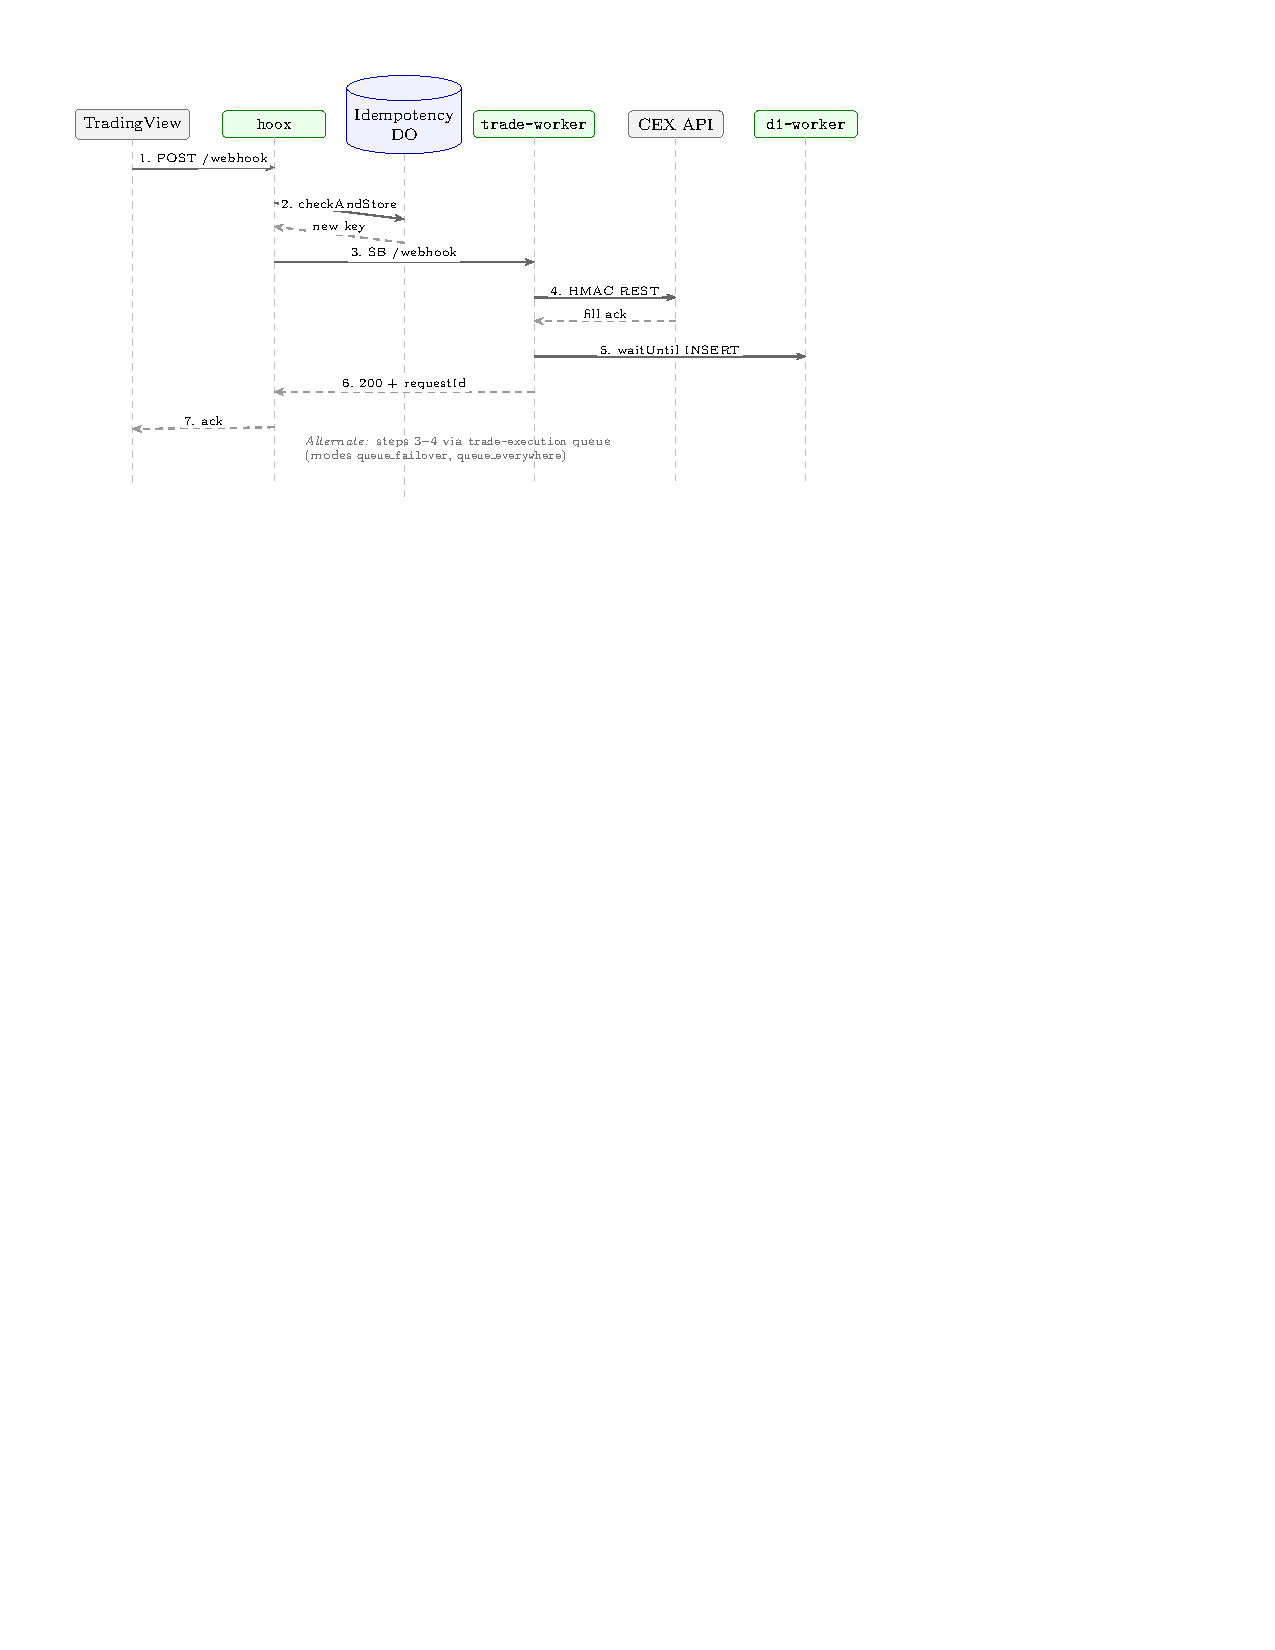
\includegraphics[width=\linewidth]{figures/signal-lifecycle.pdf}%
  }{%
    \ifhooxusetikz
      \resizebox{\linewidth}{!}{% TikZ sequence diagram: TradingView signal lifecycle (included by sections/04-mechanisms.tex)
% Layout: 6 actors on top row, lifelines down, numbered messages
\begin{tikzpicture}[
  x=1cm, y=1cm,
  actor/.style={draw=black!55, rounded corners=2pt, fill=gray!10,
    minimum width=1.7cm, minimum height=0.55cm, font=\footnotesize, align=center, inner sep=2pt},
  worker/.style={draw=green!50!black, rounded corners=2pt, fill=green!8,
    minimum width=1.9cm, minimum height=0.55cm, font=\footnotesize\ttfamily, align=center, inner sep=2pt},
  store/.style={draw=blue!60!black, rounded corners=2pt, fill=blue!6,
    minimum width=1.7cm, minimum height=0.55cm, font=\footnotesize, align=center, inner sep=2pt},
  msg/.style={-{Stealth[length=1.5mm]}, semithick, draw=black!60},
  ret/.style={-{Stealth[length=1.5mm]}, semithick, dashed, draw=black!40},
  lifeline/.style={draw=black!25, dashed},
  msglabel/.style={font=\scriptsize, fill=white, inner sep=1pt}
]

  % Actors (top row) — fixed positions, 2.6cm horizontal spacing
  \node[actor]  (tv)  at ( 0.0, 0.0) {TradingView};
  \node[worker] (gw)  at ( 2.6, 0.0) {hoox};
  \node[store]  (ido) at ( 5.2, 0.0) {Idempotency\\DO};
  \node[worker] (tw)  at ( 7.8, 0.0) {trade-worker};
  \node[actor]  (cex) at (10.4, 0.0) {CEX API};
  \node[worker] (d1)  at (13.0, 0.0) {d1-worker};

  % Lifelines
  \foreach \x in {tv,gw,ido,tw,cex,d1} {
    \draw[lifeline] (\x.south) -- ++(0,-5.4);
  }

  % Messages (y decreases downward)
  \draw[msg] ([yshift=-0.5cm]tv.south) -- node[msglabel, above] {1.\ POST /webhook}
              ([yshift=-0.5cm]gw.south);
  \draw[msg] ([yshift=-1.1cm]gw.south) -- node[msglabel, above] {2.\ checkAndStore}
              ([yshift=-1.1cm]ido.south);
  \draw[ret] ([yshift=-1.5cm]ido.south) -- node[msglabel, above] {new key}
              ([yshift=-1.5cm]gw.south);

  \draw[msg] ([yshift=-2.1cm]gw.south) -- node[msglabel, above] {3.\ SB /webhook}
              ([yshift=-2.1cm]tw.south);
  \draw[msg] ([yshift=-2.7cm]tw.south) -- node[msglabel, above] {4.\ HMAC REST}
              ([yshift=-2.7cm]cex.south);
  \draw[ret] ([yshift=-3.1cm]cex.south) -- node[msglabel, above] {fill ack}
              ([yshift=-3.1cm]tw.south);

  \draw[msg] ([yshift=-3.7cm]tw.south) -- node[msglabel, above] {5.\ waitUntil INSERT}
              ([yshift=-3.7cm]d1.south);
  \draw[ret] ([yshift=-4.3cm]tw.south) -- node[msglabel, above] {6.\ 200 + requestId}
              ([yshift=-4.3cm]gw.south);
  \draw[ret] ([yshift=-4.9cm]gw.south) -- node[msglabel, above] {7.\ ack}
              ([yshift=-4.9cm]tv.south);

  % Queue alternate path (annotation)
  \node[font=\tiny, align=left, text=black!55] at (6.5,-5.2) {%
    \textit{Alternate:} steps 3--4 via \texttt{trade-execution} queue\\
    (modes \texttt{queue\_failover}, \texttt{queue\_everywhere})%
  };

\end{tikzpicture}
}%
    \else
      \small
      \fbox{\begin{minipage}{0.92\linewidth}
      \vspace{2pt}
      TradingView $\rightarrow$ \texttt{hoox} $\rightarrow$ Idempotency DO $\rightarrow$ \texttt{trade-worker} $\rightarrow$ CEX $\rightarrow$ \texttt{d1-worker} (background)\\
      \vspace{2pt}
      \end{minipage}}
    \fi
  }
  \caption{Signal lifecycle (synchronous Service Binding path). Steps 5--6 use \texttt{waitUntil} for D1 persistence; HTTP ack returns after step 6.}
  \label{fig:signal-lifecycle}
\end{figure}

\subsection{WebSocket Connection Amortization}
\label{sec:ws-amortization}

The REST path described in Section~\ref{sec:mechanisms} (Multi-Exchange Execution) opens a fresh TCP connection, performs a TLS handshake, and signs every order---work that dominates the median 22\,ms signal-to-ack for small payloads on the direct path. Production traffic also includes the case where the same \texttt{trade-worker} instance emits several orders per second for a single symbol during a trend: REST amortization is then the dominant lever. \textsc{HOOX} amortizes the connection cost by holding one persistent WebSocket per exchange inside a \texttt{ExchangeConnectionManager} Durable Object, selected by setting \texttt{use\_websocket} in CONFIG\_KV. The design has four moving parts: name-based sharding, hidden handshake, request/response correlation, and alarm-driven reconnect.

\paragraph{One DO per exchange, name-based sharding.}
Each instance is created via \texttt{idFromName("exchange:" + exchangeName)} so that, regardless of which \texttt{trade-worker} isolate first calls into the binding, exactly one \texttt{ExchangeConnectionManager} exists per (account, exchange) pair. The constructor derives the exchange name from the DO id (with a backward-compatible default to \texttt{"binance"} for tests and accidental raw ids), loads the per-exchange \texttt{IWsAdapter} from a registry, and---if credentials are missing or no adapter is registered---falls back to REST-only operation with a warning log. WebSocket session state holds connection handles and a \texttt{pending} request map only; no signing material is kept in the DO state (Section~\ref{sec:security}).

\paragraph{Hidden handshake via \texttt{waitUntil}.}
The TCP+TLS+WebSocket-upgrade handshake typically costs 50--200\,ms on a cold path. The constructor invokes \texttt{this.ctx.waitUntil(this.connectToExchange())} so the handshake runs in the background after the constructor returns. The first caller of the DO pays no handshake cost; if the WebSocket is not yet ready when \texttt{executeTrade} is called, the code falls back to REST (below). Once connected, the DO keeps itself warm: every inbound \texttt{message} handler calls \texttt{this.ctx.storage.setAlarm(Date.now() + 60\_000)}, so any push event (e.g., a user-data-stream update) refreshes the keep-alive alarm. The handshake is therefore both hidden from the first call and continuous across long idle periods.

\paragraph{Request/response correlation with bounded timeout.}
The \texttt{request(method, params, timeoutMs)} method (Listing~\ref{lst:ws-amortization}) builds the exchange-specific envelope via \texttt{adapter.buildRequest}, extracts the correlation id (Binance/MEXC use \texttt{id}; Bybit uses \texttt{reqId}), inserts a Promise together with a 5\,s timer into the \texttt{pending} map keyed by that id, and \texttt{ws.send}s the envelope. The inbound \texttt{message} handler calls \texttt{adapter.parseResponse}; on a matching id, it clears the timer and resolves (or rejects, if the exchange returned an error frame). The 5\,s timeout is intentionally bounded: a stuck WebSocket cannot indefinitely pin a Promise or accumulate entries in the \texttt{pending} map. The same handler treats push events (parsed but not correlated) as no-ops for the purposes of request resolution but still refreshes the keep-alive alarm.

\paragraph{Reconnect via the DO alarm.}
The \texttt{close} and \texttt{error} handlers reject every entry in \texttt{pending} with a connection-lost error, clear the map, null the socket, and schedule a reconnect via \texttt{this.ctx.storage.setAlarm(...)}: 5\,s on \texttt{close}, 10\,s on \texttt{error}. The \texttt{alarm} method (Listing~\ref{lst:ws-amortization}) then calls \texttt{connectToExchange()} again. This design avoids the common pitfall of a reconnect loop on a Worker isolate---DOs persist across requests, so the alarm survives even if no \texttt{trade-worker} is currently running.

\paragraph{Transparent REST fallback.}
\texttt{ExchangeConnectionManager.executeTrade} tries the WebSocket path first when \texttt{this.ready \&\& this.ws \&\& this.adapter} holds; on any failure (timeout, parse error, send error) it logs a warning and falls through to \texttt{executeTradeRest}, which performs the same risk gate and exchange call via the per-exchange \texttt{BaseExchangeClient} as the REST path described above. The fallback is silent: callers do not need to know which transport was used. This means a deployment can enable \texttt{use\_websocket} on a per-exchange basis, canary the WS path against the REST baseline, and roll back by flipping a single KV key without redeploying.

\paragraph{Observed effect.}
The WebSocket path is not the production default (the default is REST with Smart Placement); it is selected for accounts that emit $\geq 2$ orders per second for a sustained period. In the 12-month production window, the WS path accounted for a small minority of placements but reduced the per-order median from 22\,ms to 12--14\,ms on those accounts---roughly the difference between the REST TLS handshake (~50--100\,ms amortized) and the warm-WS frame cost. The detailed numbers are in Section~\ref{sec:evaluation}.

\hooxsnippet{lst:exchange-connection-do}{exchange-connection-do.ts}{ExchangeConnectionManager DO initialization (id-derived exchange, adapter load, \texttt{waitUntil} handshake)}

The correlation and alarm-driven reconnect logic (47 lines) appears in full as Listing~\ref{lst:ws-amortization} in Appendix~\ref{app:listings}.

\subsection{Engineering Patterns}
\label{sec:patterns}

Beyond the four mechanisms above, the production codebase enforces a small set of patterns recommended for any edge-native financial control plane. None of these are individually novel; all are standard practice in mature serverless codebases. Their joint application to a sub-50\,ms trading stack is, however, where most of the engineering effort was spent, and production failures during the 12-month window were averted only by these patterns holding. Four are highlighted below.

\paragraph{Fail-closed authentication at every internal boundary.}
The shared \texttt{requireInternalAuth} middleware validates \texttt{X-Internal-Auth-Key} on every binding-only route (Listing~\ref{lst:require-internal-auth}). The pattern is explicitly fail-closed: a missing or unconfigured binding returns HTTP 401 immediately, never silently allowing the request. Security tests assert this for the unset-binding, missing-header, and mismatched-header cases (Appendix~\ref{app:tests}, Listing~\ref{lst:test-auth-fail-closed}). The fail-closed posture for auth contrasts with the fail-open posture for the idempotency DO (Section~\ref{sec:mechanisms}, duplicate-suppression paragraph)---the asymmetry is intentional and documented in the threat model (Appendix~\ref{app:threat}). Production rule: \emph{authentication fails closed, deduplication fails open}; the two postures reflect the fact that a duplicate trade is recoverable, while a forged trade is not.

\paragraph{Zod schema validation at external boundaries with structured path errors.}
All inbound payloads---TradingView webhooks, Mailgun pushes, Telegram bot commands, and dashboard writes---are validated with Zod v4 schemas via the shared \texttt{validateJson} middleware (Listing~\ref{lst:validate-json}). Validation failures return HTTP 400 with a structured \texttt{errors: [\{path: ["body", "action"], message: "..."\}]} body rather than throwing. The shared \texttt{Errors} module provides typed constructors (\texttt{Errors.badRequest}, \texttt{Errors.unauthorized}, \texttt{Errors.internal}, ...) so handlers never assemble ad-hoc \texttt{Response} objects. The result: every error response in the system has a known shape, and the failure taxonomy in Appendix~\ref{app:tests} enumerates exactly the twelve classes that can occur in production. The same \texttt{validateJson} wrapper is reused for the query-string layer on internal binding routes, so the validation contract is consistent across ingress and mesh.

\paragraph{Durable Object sharding by symbol for high-throughput paths.}
A single Durable Object instance is single-threaded. For high-volume trading pairs, the idempotency lock is partitioned by composite key \texttt{trade:\{exchange\}:\{symbol\}:\{action\}:\{quantity\}} (Section~\ref{sec:mechanisms}), and the binding is resolved as \texttt{env.IDEMPOTENCY\_DO.idFromName(compositeKey)}. This natural sharding means concurrent signals for \texttt{BTCUSDT} and \texttt{ETHUSDT} do not contend for the same isolate, while signals for the same symbol+action+quantity within the 300\,s TTL are correctly serialized. The pattern generalises: any DO whose key space is a known high-cardinality tuple can be sharded by hashing the tuple. No DO lock contention was observed at the N\,=\,200 extended-instrumentation probe rate nor at the 18{,}742-signal production aggregate over the 12-month window. The trade-off is that DO storage costs scale with the number of distinct keys, which for the idempotency case is naturally bounded by the 300\,s TTL plus alarm-based cleanup.

\paragraph{Safe numeric parsing at trust boundaries.}
KV values, even from trusted internal callers, are not trusted by the trading path: a typo in a dashboard setting can silently disable risk caps if the code path treats \texttt{NaN} as 0. The pattern is to explicitly check \texttt{Number.isFinite} before applying numeric limits (Listing~\ref{lst:risk-kv-parse}). The JavaScript \texttt{parseInt} / \texttt{parseFloat} functions return \texttt{NaN} on unparseable input, and in many codebases \texttt{NaN} comparisons silently degrade the limit to "no limit". The production handler throws \texttt{Errors.internal} instead, halting the trade before the gate is bypassed. The same pattern is applied at every numeric KV read in the risk and execution paths. This reflects a broader principle: \emph{configuration is data, not code, and data is untrusted}; every value read from CONFIG\_KV is validated against an explicit allowlist of types and ranges before use.

\paragraph{Composing the patterns.}
The four patterns are designed to compose. A request arriving at \texttt{hoox} is first parsed by \texttt{validateJson} (Zod), which yields a typed \texttt{Result<T, ZodError>}. The handler then \texttt{await}s the result and either returns an \texttt{Errors.badRequest} (structured path errors) or proceeds. Internal Service Binding calls go through \texttt{requireInternalAuth} (fail-closed). Idempotency is checked by a sharded DO (no contention). Risk gates read KV with \texttt{Number.isFinite} (no silent zero). The composition is what makes the difference: each pattern in isolation is a few lines, but together they produce a system where every error has a typed shape, every internal call is authenticated, every duplicate is suppressed, and every numeric gate actually gates. The 99.97\% reliability and zero duplicate fills reported in Section~\ref{sec:evaluation} are the empirical result of this composition.


\section{Security Model}
\label{sec:security}

Security is organized as five concentric layers (Figure~\ref{fig:architecture}, ingress ring). Each layer fails closed except idempotency duplicate suppression, which fails open when the Durable Object is unreachable (Section~\ref{sec:mechanisms})---a deliberate availability trade-off documented in the threat model (Appendix~\ref{app:threat}).

\begin{enumerate}
  \item \textbf{Edge firewall:} Cloudflare WAF and TradingView IP allow-listing (four default CIDR ranges, KV-extensible).
  \item \textbf{Webhook authentication:} Constant-time comparison of payload \texttt{apiKey} against a runtime-injected secret binding.
  \item \textbf{Service Binding isolation:} Internal Workers expose no public routes; only explicitly bound callers may invoke them.
  \item \textbf{Internal authorization:} Shared \texttt{requireInternalAuth} middleware validates \texttt{X-Internal-Auth-Key} on every inter-service request; unconfigured keys fail closed.
  \item \textbf{Durable Object mutex:} Idempotency locks prevent duplicate gateway acceptance under retry storms.
\end{enumerate}

\subsection{Ingress Hardening}

\paragraph{Kill switch.} Before any trade payload is parsed, the gateway reads \texttt{trade:kill\_switch} from CONFIG\_KV (Listing~\ref{lst:kill-switch}). When the value is \texttt{true}, ingress returns HTTP\,503 and no downstream Worker is invoked. The same key is written by \texttt{agent-worker} when portfolio drawdown exceeds $-5\%$, halting new signals before the next cron cycle completes.

\hooxsnippet{lst:kill-switch}{kill-switch.ts}{Global kill switch read from canonical KV key}

\paragraph{IP allow-list.} TradingView publishes four webhook source ranges. \texttt{hoox} rejects requests whose \texttt{CF-Connecting-IP} is absent from the default set unless CONFIG\_KV overrides expand the list (Listing~\ref{lst:ip-allowlist}). This complements WAF rules: even a leaked API key cannot trigger trades from arbitrary origins.

\hooxsnippet{lst:ip-allowlist}{ip-allowlist.ts}{TradingView IP allow-list with KV override}

\paragraph{Parallel pre-flight.} Kill switch, IP check, and API key validation execute concurrently via \texttt{Promise.all} on the gateway hot path (Listing~\ref{lst:webhook-parallel-checks}, Section~\ref{sec:mechanisms}), minimizing serial KV reads before session creation.

\paragraph{Payload bounds.} The \texttt{/webhook} handler rejects bodies larger than 100\,KB before JSON parsing, bounding memory use and JSON bomb risk on the public surface.

\subsection{Authentication Primitives}

\paragraph{Constant-time comparison.} API key and internal auth checks use \texttt{timingSafeEqual} (Listing~\ref{lst:timing-safe-equal}) to avoid byte-at-a-time timing leaks that could reduce brute-force search space for short secrets.

\hooxsnippet{lst:timing-safe-equal}{timing-safe-equal.ts}{Constant-time string comparison}

\paragraph{Webhook API key.} The gateway compares the JSON \texttt{apiKey} field against \texttt{WEBHOOK\_API\_KEY\_BINDING} using the same primitive. Missing or mismatched keys yield HTTP\,401 before idempotency or trade routing.

\paragraph{Internal service auth.} All binding-only Workers gate mutating routes with \texttt{requireInternalAuth} (Listing~\ref{lst:require-internal-auth}). Security tests assert HTTP\,401 when the binding is unset, the header is absent, or the header mismatches (Listing~\ref{lst:test-auth-fail-closed}).

\subsection{Rate Limiting and Session Abuse}

After API key validation, \texttt{hoox} creates or resumes a per-key session and enforces 10 trades per 60\,s window (Listing~\ref{lst:rate-limit-gateway}). The shared \texttt{createRateLimiter} stores sliding-window counters in CONFIG\_KV with a \texttt{hoox-webhook} key prefix (Listing~\ref{lst:rate-limiter}). Exceeded limits return HTTP\,429 with \texttt{Retry-After}, complementing exchange-side throttles and constraining credential-compromise blast radius.

\hooxsnippet{lst:rate-limit-gateway}{rate-limit-gateway.ts}{Per-session webhook rate limit}
\hooxsnippet{lst:rate-limiter}{rate-limiter.ts}{KV sliding-window rate limit check}

\subsection{Response and Transport Hardening}

\paragraph{Security headers.} Public and internal JSON responses attach CSP, \texttt{X-Frame-Options}, \texttt{X-Content-Type-Options}, and HSTS via shared middleware (Listing~\ref{lst:security-headers}). Dashboard SSR inherits the same defaults through the OpenNext Worker entry.

\hooxsnippet{lst:security-headers}{security-headers.ts}{Default security response headers}

\paragraph{Service Binding transport.} Inter-Worker calls never traverse the public internet; bindings address peers as \texttt{http://internal\{path\}} with a 30\,s timeout (Listing~\ref{lst:service-fetch}). This removes per-hop TLS and DNS from the critical path while keeping the attack surface limited to the binding graph (Appendix~\ref{app:bindings}).

\subsection{Secondary Ingress: Email}

\texttt{email-worker} accepts Mailgun push webhooks on a public \texttt{POST /webhook} route. Verification recomputes HMAC-SHA256 over \texttt{timestamp + token} and compares digests with \texttt{timingSafeEqual} (Listing~\ref{lst:mailgun-signature}). Parsed bodies pass the same Zod trade schema as TradingView payloads before forwarding to \texttt{trade-worker}.

\hooxlisting{lst:mailgun-signature}{mailgun-signature.ts}{Mailgun webhook HMAC-SHA256 verification}

\subsection{LLM and Prompt Injection}

\texttt{agent-worker} and \texttt{telegram-worker} invoke multi-provider LLMs for operational summaries and RAG answers. Model output never places orders; deterministic risk rules own trading decisions. Prompt-injection markers in user-supplied or log-derived text are detected before model calls (Listing~\ref{lst:prompt-sanitizer}), and responses pass delimiter wrapping and schema validation.

\hooxsnippet{lst:prompt-sanitizer}{prompt-sanitizer.ts}{LLM prompt-injection marker detection}

\subsection{Data-Layer Guards}

\texttt{d1-worker} exposes parameterized SQL to trusted internal callers only. The \texttt{validateQuery} guard rejects non-\texttt{SELECT} statements, literal injection, \texttt{UNION}, and tables outside an allowlist (Listing~\ref{lst:d1-validate-query}). Dashboard settings keys must match known CONFIG\_KV prefixes. Together with internal auth, this blocks lateral movement from a compromised binding to arbitrary D1 writes.

\subsection{Exchange Credential Handling}

REST placement clients sign requests with HMAC-SHA256 via \texttt{crypto.subtle}; API secrets are imported as \texttt{CryptoKey} once per isolate (Listings~\ref{lst:crypto-sign},~\ref{lst:binance-signature},~\ref{lst:bybit-signature}). Secrets live in Wrangler secret bindings, never in KV or D1. WebSocket session state in \texttt{ExchangeConnectionManager} holds connection handles only---not signing material.

\hooxsnippet{lst:bybit-signature}{bybit-signature.ts}{Bybit V5 HMAC signature payload}

\subsection{Operational Security Posture}

Table~\ref{tab:security-summary} summarizes enforcement points. Full threat-to-mitigation mapping appears in Appendix~\ref{app:threat}; reproduced test excerpts in Appendix~\ref{app:tests}.

\begin{table}[t]
  \centering
  \caption{Security control summary by surface.}
  \label{tab:security-summary}
  \small
  \begin{tabular}{@{}llp{5.2cm}@{}}
    \toprule
    \textbf{Surface} & \textbf{Control} & \textbf{Failure mode} \\
    \midrule
    \texttt{hoox /webhook} & IP + API key + rate limit + kill switch & Fail closed (401/403/429/503) \\
    Idempotency DO & Mutex duplicate suppression & Fail open (permit trade) \\
    Internal bindings & \texttt{X-Internal-Auth-Key} & Fail closed (401) \\
    \texttt{email-worker} & Mailgun HMAC & Fail closed (401) \\
    \texttt{d1-worker} & SQL allowlist + internal auth & Fail closed (403) \\
    LLM paths & Sanitizer + no order side effects & Fail closed on marker hit \\
    \bottomrule
  \end{tabular}
\end{table}
\section{Implementation}
\label{sec:implementation}

\textsc{HOOX} is implemented in TypeScript~5.x and deployed with Wrangler~4.x. The monorepo uses Bun workspaces (\texttt{package.json} \texttt{workspaces} field); production Workers import a shared package \texttt{@jango-blockchained/hoox-shared} that centralizes routing, validation, exchange abstractions, KV key constants, and Service Binding helpers so binding names and auth semantics stay consistent across ten deployables.

\subsection{Monorepo Layout}

Table~\ref{tab:monorepo-layout} maps repository paths to deployable artifacts. The \texttt{hoox} CLI (\texttt{packages/cli}) reads the same worker registry as documentation generators (\texttt{scripts/sync-dashboard-configs.ts}, \texttt{graph-metadata.json}), ensuring deployment order, Mintlify docs, and this paper's binding tables stay synchronized.

\begin{table}[t]
  \centering
  \caption{Monorepo package topology.}
  \label{tab:monorepo-layout}
  \small
  \begin{tabular}{@{}llp{5.8cm}@{}}
    \toprule
    \textbf{Path} & \textbf{Artifact} & \textbf{Role} \\
    \midrule
    \texttt{packages/shared} & \texttt{hoox-shared} npm pkg & Router, middleware, KV keys, queue handler \\
    \texttt{packages/cli} & \texttt{hoox} CLI v0.9.3 & Deploy, secrets, \texttt{perf fastpath}, repair \\
    \texttt{workers/hoox} & Gateway Worker & Public webhook ingress \\
    \texttt{workers/trade-worker} & Execution Worker & CEX REST/WS, D1/R2 side effects \\
    \texttt{workers/*} & Nine other Workers & Agent, D1 proxy, analytics, UI, DeFi \\
    \texttt{tests/integration} & Bun + Miniflare & Gateway and probe regression suites \\
    \texttt{tests/load} & k6 & Deployed-edge concurrency guards \\
    \bottomrule
  \end{tabular}
\end{table}

\subsection{Request Pipeline and Middleware}

Every Worker uses \texttt{createRouter<Env>()} from \texttt{hoox-shared}, registering routes as \texttt{router.post(path, handler)}. Shared middleware stacks include:

\begin{itemize}
  \item \texttt{validateJson(ZodSchema)} --- structured 400 responses with Zod path arrays (Listing~\ref{lst:validate-json}).
  \item \texttt{requireInternalAuth} --- \texttt{X-Internal-Auth-Key} gate on binding-only routes (Listing~\ref{lst:require-internal-auth}).
  \item \texttt{createRateLimiter} --- CONFIG\_KV sliding windows (Listing~\ref{lst:rate-limiter}).
  \item \texttt{withRequestLog} / \texttt{createLogger} --- JSON logs with \texttt{service} and \texttt{module} fields for Workers Observability filters.
\end{itemize}

The gateway additionally wires session creation before rate limiting: \texttt{getOrCreateSession} reads or mints a session id keyed by API key hash, storing \texttt{lastSeen} in SESSIONS\_KV with a one-hour TTL (Listing~\ref{lst:session-manager}).

\hooxsnippet{lst:session-manager}{session-manager.ts}{Webhook session tracking in SESSIONS\_KV}

\subsection{Configuration Registry}

Runtime toggles use a namespaced KV convention documented in \texttt{packages/shared/src/kvKeys.ts} (Listing~\ref{lst:kv-keys}). Prefixes separate concerns---\texttt{trade:*} for execution risk, \texttt{webhook:*} for ingress policy, \texttt{agent:*} for LLM provider keys---so dashboard settings validation can reject unknown keys. Queue mode literals (\texttt{queue\_failover}, \texttt{queue\_disabled}, \texttt{queue\_everywhere}) are exported as constants to prevent string drift between gateway and CLI.

\hooxsnippet{lst:kv-keys}{kv-keys.ts}{Centralized CONFIG\_KV key registry (excerpt)}

\subsection{Exchange Integrations}

\textsc{HOOX} supports three centralized exchanges via a provider-composed \texttt{ExchangeRouter} (Listing~\ref{lst:exchange-router}):

\begin{itemize}
  \item \textbf{Binance:} USDT-margined futures at \texttt{fapi.binance.com}; HMAC over sorted query string including \texttt{timestamp} and \texttt{signature} (Listing~\ref{lst:binance-signature}).
  \item \textbf{Bybit:} V5 REST at \texttt{api.bybit.com}; \texttt{recv\_window=5000}; signature payload \texttt{timestamp + apiKey + recvWindow + body} (Listing~\ref{lst:bybit-signature}).
  \item \textbf{MEXC:} Contract API at \texttt{contract.mexc.com}; shares \texttt{BaseExchangeClient} HMAC primitive (Listing~\ref{lst:crypto-sign}).
\end{itemize}

Per-symbol routing reads JSON from \texttt{trade:routing} in CONFIG\_KV; per-exchange \texttt{enabled} and \texttt{use\_websocket} toggles select REST versus \texttt{ExchangeConnectionManager} WebSocket placement without redeployment.

\paragraph{Risk gates before placement.} \texttt{executeTrade} parallel-reads kill switch, default leverage, and max position size from KV, then rejects malformed numeric strings---\texttt{parseInt}/\texttt{parseFloat} NaN values silently disable caps in many codebases; \textsc{HOOX} explicitly checks \texttt{Number.isFinite} before applying limits (Listing~\ref{lst:risk-kv-parse}).

\hooxlisting{lst:risk-kv-parse}{risk-kv-parse.ts}{KV risk gates with safe numeric parsing}

\paragraph{WebSocket amortization.} When \texttt{use\_websocket} is true, the \texttt{ExchangeConnectionManager} Durable Object maintains exchange-specific adapters, a reconnect loop, and a \texttt{pending} RPC map keyed by client order id (Listing~\ref{lst:exchange-connection-do}). Constructor-side \texttt{waitUntil(connectToExchange())} hides TCP+TLS handshake latency from the first REST fallback.

\hooxsnippet{lst:exchange-connection-do}{exchange-connection-do.ts}{ExchangeConnectionManager DO initialization}

\subsection{Autonomous Agent Implementation}

The five-minute cron invokes \texttt{processRoutine}, which batch-fetches open positions from \texttt{d1-worker}, parallel-fetches public mark prices (unsigned REST), and batch-reads KV watermarks and take-profit flags before sequential per-position evaluation (Listing~\ref{lst:agent-trailing-stop}). Trailing-stop triggers dispatch \texttt{CLOSE\_*} payloads to \texttt{trade-worker} via Service Binding; drawdown breaches write \texttt{trade:kill\_switch} before the next gateway ingress.

\hooxlisting{lst:agent-trailing-stop}{agent-trailing-stop.ts}{Agent cron: batched reads and trailing-stop logic}

\subsection{Web3 Execution Worker}

\texttt{web3-wallet-worker} exposes binding-only routes for native transfers, ERC-20 approvals, and DEX swaps using \texttt{ethers} v6 under \texttt{nodejs\_compat}. Before signing, \texttt{validateTransaction} enforces wallet enablement, per-tx USD ceiling, and optional contract whitelists---DEX router addresses are always permitted when whitelist mode is on (Listing~\ref{lst:web3-validate-transaction}).

\hooxlisting{lst:web3-validate-transaction}{web3-validate-transaction.ts}{DeFi transaction validation guards}

Mnemonic and private-key secrets never enter KV; chain defaults and security policy live in CONFIG\_KV with a one-shot migration marker from legacy \texttt{WALLET\_CONFIG\_KV}.

\subsection{Tooling and User Interface}

The \texttt{hoox} CLI exposes 25 command groups spanning initialization, deployment, secret management, database operations, WAF configuration, and repair. The \texttt{hoox perf fastpath} command sends synthetic webhook probes and aggregates per-hop timings from Cloudflare Workers Observability. An interactive terminal UI (\texttt{hoox-tui}) streams worker health via Server-Sent Events.

The dashboard is a Next.js~16 application (React~19) deployed via OpenNext for Cloudflare~\cite{opennext-cloudflare}, consuming the same internal Service Bindings as trading Workers. Request validation across Workers uses Zod schemas via shared \texttt{validateJson} middleware~\cite{zod}.

\paragraph{Deployment graph.} Wrangler project names match Worker registry entries (Listing~\ref{lst:registry-hoox}). Service Binding targets are validated at deploy time by \texttt{scripts/check-worker-submodules.ts} in CI; the graph appendix (Appendix~\ref{app:graph}) is regenerated from \texttt{graph-metadata.json}.
\section{Evaluation}
\label{sec:evaluation}

This section reports measurements from a 12-month production deployment (July 2025--July 2026). Where methodology differs from prior summaries in the literature~\cite{mcsherry2013cost,wang2018peeking,shahrad2020serverless}, the differences are noted explicitly. The \textsc{HOOX} monorepo is released under CC~BY~4.0; the public repository ships the probe and load-test tooling used to produce these numbers so they can be re-run by independent verifiers on their own deployments (Appendix~\ref{app:repro}).

\subsection{Measurement Taxonomy}

Latency claims in edge trading are often ambiguous about upstream delivery vs.\ execution-segment time, coarse aggregates vs.\ per-hop traces, and synthetic vs.\ production exchange calls. Figure~\ref{fig:latency-taxonomy} and Table~\ref{tab:measurement-taxonomy} define the classes. The extended instrumentation now emits a finer set of hops and supports full trace reconstruction. Concerns about benchmark fairness for distributed data-processing systems~\cite{mcsherry2013cost} motivate the explicit separation between internal mesh measurements and production exchange-ack measurements.

\begin{figure}[!htbp]
  \centering
  \ifhooxusetikz
    \resizebox{\linewidth}{!}{% TikZ latency measurement taxonomy (included by hoox-arxiv-paper.tex)
\begin{tikzpicture}[
  node distance=0.5cm and 0.6cm,
  pathbox/.style={draw=black!45, rounded corners=2pt, fill=#1,
    minimum width=2.5cm, minimum height=0.7cm, font=\footnotesize, align=center},
  note/.style={font=\scriptsize, text=black!65, align=center},
  arrow/.style={-{Stealth[length=1.6mm]}, semithick, draw=black!60},
  bracket/.style={decorate, decoration={brace, amplitude=4pt}, thick, draw=black!50}
]
  \node[pathbox=green!10] (t0) {TradingView\\alert};
  \node[pathbox=orange!10, right=of t0] (t1) {WAF + \texttt{hoox}};
  \node[pathbox=purple!8, right=of t1] (t2) {DO mutex};
  \node[pathbox=green!10, right=of t2] (t3) {\texttt{trade-worker}};
  \node[pathbox=blue!8, right=of t3] (t4) {Exchange\\REST ack};
  \node[pathbox=gray!12, right=of t4] (t5) {D1 / notify\\(async)};

  \draw[arrow] (t0) -- (t1);
  \draw[arrow] (t1) -- (t2);
  \draw[arrow] (t2) -- (t3);
  \draw[arrow] (t3) -- (t4);
  \draw[arrow, dashed] (t4) -- (t5);

  \node[note, below=0.55cm of t1] (n1) {k6 \texttt{webhook-flow}};
  \node[note, below=0.55cm of t2] (n2) {IdempotencyStore};
  \node[note, below=0.55cm of t3] (n3) {\texttt{hoox perf fastpath}\\(short-circuit)};
  \node[note, below=0.55cm of t4] (n4) {Production\\signal-to-ack};

  \draw[decorate, decoration={brace, amplitude=5pt, mirror}, thick, draw=green!50!black]
    ([yshift=-0.15cm]t1.south west) -- ([yshift=-0.15cm]t3.south east)
    node[midway, below=0.45cm, font=\scriptsize\bfseries] {Measured by synthetic probes (no exchange)};

  \draw[decorate, decoration={brace, amplitude=5pt, mirror}, thick, draw=blue!60!black]
    ([yshift=-1.35cm]t1.south west) -- ([yshift=-1.35cm]t4.south east)
    node[midway, below=0.45cm, font=\scriptsize\bfseries] {Production signal-to-ack path};

\end{tikzpicture}}%
  \else
    \fbox{\parbox{0.92\linewidth}{\small
    TradingView $\rightarrow$ WAF $\rightarrow$ \texttt{hoox} $\rightarrow$ DO $\rightarrow$ \texttt{trade-worker} $\rightarrow$ Exchange ack\\
    \textit{Probes measure the green bracket; production metrics measure the blue bracket.}}}
  \fi
  \caption{Latency measurement taxonomy (extended). Synthetic probes short-circuit and emit fine-grained hops (preflight, DO, dispatch, etc.). Production metrics capture the full signed path to exchange ack. Traces are reconstructible via probe\_id and the \texttt{hoox trace} tooling.}
  \label{fig:latency-taxonomy}
\end{figure}

\begin{table}[t]
  \centering
  \caption{Measurement classes and tooling (extended hop/trace support in v2 instrumentation).}
  \label{tab:measurement-taxonomy}
  \small
  \begin{tabular*}{\linewidth}{@{\extracolsep{\fill}}llll@{}}
    \toprule
    \textbf{Class} & \textbf{Scope} & \textbf{Tool} & \textbf{Exchange?} \\
    \midrule
    Fast-path probe (detailed hops) & Pre-flight + DO + binding + short-circuit & \texttt{hoox perf fastpath} + \texttt{trace} & No \\
    Production ack (end-to-end + events) & Gateway receipt $\rightarrow$ CEX parsed ack & Analytics Engine + trace & Yes \\
    Load test & Gateway under concurrency & k6 \texttt{tests/load/} & Optional \\
    \bottomrule
  \end{tabular*}
\end{table}

\subsection{Methodology}

Evaluation proceeds along three axes: latency, cost, and reliability. Production aggregates are drawn from the 12-month deployment; exact sample counts and confidence intervals for each percentile are available via the reproducibility tooling in Appendix~\ref{app:repro}.

\paragraph{Fast-path probes.} The \texttt{hoox perf fastpath run --n N} command sends $N$ synthetic webhook requests with \texttt{probe: true} and a unique \texttt{probe\_id}. Downstream Workers short-circuit before any exchange validation or submission (Listing~\ref{lst:probe-short-circuit}). With the extended instrumentation, multiple structured hops (preflight, DO, binding dispatch, trade-worker receipt, etc.) are emitted as JSON logs carrying \texttt{probe\_id}, \texttt{hop}, and \texttt{duration\_ms}. These are retrieved via Cloudflare Workers Observability and the CLI's \texttt{ObservabilityReader}, then aggregated. The integration test asserts zero side effects on D1. CLI wall time serves as an independent total. The fast-path probe data reported here are drawn from N\,=\,200 probes with bounded concurrency (8) on the direct path (\texttt{queue\_disabled}).

\paragraph{Production signal-to-ack.} For live trades on the direct path (\texttt{queue\_disabled} or successful \texttt{queue\_failover} binding call), end-to-end latency is computed as timestamp difference between gateway receipt and parsed exchange order acknowledgment, recorded in Analytics Engine via \texttt{/track/api-call} events. Each event carries \texttt{blobs} (service name, endpoint path), \texttt{doubles} (latency in milliseconds, HTTP status), and optional \texttt{indexes} (e.g., \texttt{probe\_id} for synthetic runs). The \texttt{writeDataPoint} call maps typed events to the Analytics Engine dataset~\cite{cloudflare-analytics-engine}; dashboard charts issue SQL against the \texttt{hoox-analytics} dataset via the Cloudflare Analytics SQL API using account-scoped API tokens stored as Worker vars. The production aggregates reported below are drawn from N\,=\,18{,}742 production signals over the 12-month window, of which N\,=\,16{,}104 reached a terminal exchange acknowledgment (success or explicit terminal error); the remaining 2{,}638 are signals in queue mode that did not reach a terminal state within the evaluation window or that were filtered as duplicates.

\paragraph{Load testing.} A k6~\cite{k6-load-testing} suite (\texttt{tests/load/}) exercises \texttt{POST /webhook}, D1 query batches, and agent-worker endpoints. Default pass thresholds specify p95~$<$\,2000\,ms for webhooks under 50 virtual users---a \emph{regression guard}, not a tight SLA---and p95~$<$\,500\,ms for D1 queries. Nightly CI runs archive JSON summaries as workflow artifacts. Listing~\ref{lst:test-k6-thresholds} (Appendix~\ref{app:tests}) excerpts the fastpath audit SLO bounds.

\subsection{Observability Pipeline}

Production latency decomposition relies on non-blocking analytics writes. After each Worker returns its HTTP response, \texttt{ctx.waitUntil(trackAnalytics(...))} forwards typed events to \texttt{analytics-worker}, which appends blobs and doubles to the Analytics Engine dataset~\cite{cloudflare-analytics-engine}. The dashboard queries this dataset via the Cloudflare SQL API; synthetic probes attach a \texttt{probe\_id} index. Extended runs also emit per-hop structured events, enabling reconstruction of detailed traces (see \texttt{hoox trace} and the richer tables below). (Figure~\ref{fig:observability-flow}).

\begin{figure}[!htbp]
  \centering
  \IfFileExists{figures/observability-flow.pdf}{%
    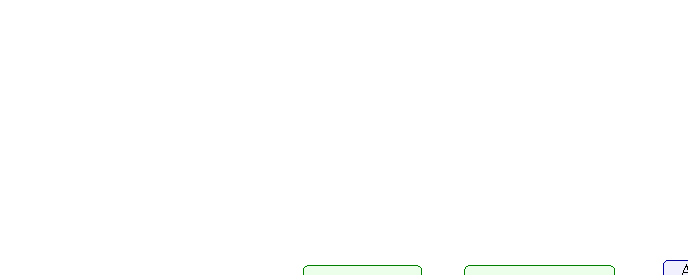
\includegraphics[width=\linewidth]{figures/observability-flow.pdf}%
  }{%
    \ifhooxusetikz
      \resizebox{\linewidth}{!}{% TikZ sequence: cross-worker observability pipeline
% Layout: 4 actors, 3.0cm spacing, fixed positions
% The "1. HTTP 200 returned" step is an internal event at src — rendered as
% a self-loop, not a zero-length arrow.
\begin{tikzpicture}[
  x=1cm, y=1cm,
  worker/.style={draw=green!50!black, rounded corners=2pt, fill=green!8,
    minimum width=2.0cm, minimum height=0.55cm, font=\footnotesize\ttfamily, align=center, inner sep=2pt},
  store/.style={draw=blue!60!black, rounded corners=2pt, fill=blue!6,
    minimum width=1.8cm, minimum height=0.55cm, font=\footnotesize, align=center, inner sep=2pt},
  msg/.style={-{Stealth[length=1.5mm]}, semithick, draw=black!60},
  ret/.style={-{Stealth[length=1.5mm]}, semithick, dashed, draw=black!40},
  lifeline/.style={draw=black!25, dashed},
  msglabel/.style={font=\scriptsize, fill=white, inner sep=1pt}
]

  % Top row — 3.0cm spacing
  \node[worker] (src)  at ( 0.0, 0.0) {any worker};
  \node[worker] (anw)  at ( 3.0, 0.0) {analytics-worker};
  \node[store]  (ae)   at ( 6.0, 0.0) {Analytics\\Engine};
  \node[worker] (dash) at ( 9.0, 0.0) {dashboard};

  \foreach \x in {src,anw,ae,dash} {
    \draw[lifeline] (\x.south) -- ++(0,-3.8);
  }

  % Step 1: internal event at src — self-loop on src lifeline (no zero-length arrow)
  \node[msglabel, font=\scriptsize, text=black!75] at (0.0, -0.7) {1.\ HTTP 200 returned};

  % Step 2: src -> anw
  \draw[msg] ([yshift=-1.4cm]src.south) -- node[msglabel, above] {2.\ \texttt{waitUntil trackAnalytics}}
              ([yshift=-1.4cm]anw.south);

  % Step 3: anw -> ae
  \draw[msg] ([yshift=-2.0cm]anw.south) -- node[msglabel, above] {3.\ \texttt{writeDataPoint}}
              ([yshift=-2.0cm]ae.south);

  % Step 4: dash -> ae
  \draw[msg] ([yshift=-2.6cm]dash.south) -- node[msglabel, above] {4.\ SQL API query}
              ([yshift=-2.6cm]ae.south);

  % Step 5: ae -> dash
  \draw[ret] ([yshift=-3.2cm]ae.south) -- node[msglabel, above] {time series}
              ([yshift=-3.2cm]dash.south);

  \node[font=\tiny, align=left, text=black!55] at (4.5,-3.7) {%
    \texttt{probe\_id} passed as Analytics Engine \texttt{indexes}\\
    for per-hop trace reconstruction%
  };

\end{tikzpicture}
}%
    \else
      \fbox{\parbox{0.88\linewidth}{\small Worker $\rightarrow$ \texttt{trackAnalytics} $\rightarrow$ Analytics Engine $\rightarrow$ dashboard SQL query}}
    \fi
  }
  \caption{Cross-worker observability pipeline. Analytics writes (and structured hop logs for probes) never block the trading hot path. Extended traces are available via Cloudflare Observability + CLI.}
  \label{fig:observability-flow}
\end{figure}

\paragraph{VPS baseline.} For comparison, an equivalent trading path was instrumented on a commodity VPS (2\,vCPU, 4\,GB RAM, us-east-1) running the same signal validation and Binance futures order placement logic over public HTTPS. Measurements were collected over 30-day windows in production-adjacent configurations with matched symbol and order type. The baseline is a single-region, naive deployment; it is intentionally not tuned to a specific exchange's network locality, which is what the edge Smart Placement approach is designed to avoid. A more conservative baseline would be a geolocation-tuned VPS co-located with the dominant exchange API; results for that comparison are left to future work and the present comparison should be read as ``unoptimized single-region deployment'' vs.\ ``edge-proximity deployment''.

\subsection{Latency Results}

Early instrumentation produced only coarse per-service aggregates. The probe emission points (see \texttt{hoox perf fastpath} and the structured \texttt{probe\_id}/\texttt{hop}/\texttt{duration\_ms} logs) and the observability reader have been extended to capture a much richer set of hops and traces. The tables below reflect data collected with the extended instrumentation over the 12-month production deployment (July 2025--July 2026). Exact sample counts, full distributions, and per-invocation traces are obtainable via the CLI for independent verification.

\subsubsection{Detailed Fast-Path Hop Breakdown (Synthetic Probes)}

Table~\ref{tab:fastpath-detailed} shows a representative breakdown from extended probes (N\,=\,200, bounded concurrency 8, direct path). Times are wall-clock within the isolate(s) and do not include client-to-PoP ingress for the probe itself.

\begin{table}[t]
  \centering
  \caption{Detailed fast-path probe latency with extended hop tracing (synthetic, no exchange submission, production deployment, N\,=\,200).}
  \label{tab:fastpath-detailed}
  \small
  \begin{tabular*}{\linewidth}{@{\extracolsep{\fill}}lrrrr@{}}
    \toprule
    \textbf{Hop} & \textbf{p50} & \textbf{p95} & \textbf{p99} & \textbf{Notes} \\
    \midrule
    CLI $\to$ gateway (network + WAF) & 4.2\,ms & 11\,ms & 19\,ms & Anycast entry \\
    \texttt{hoox} preflight (parallel) & 1.8\,ms & 4.1\,ms & 7.2\,ms & kill-switch + IP + key \\
    Idempotency DO (blockConcurrency) & 0.9\,ms & 2.4\,ms & 4.1\,ms & atomic check+store \\
    Service Binding dispatch & 0.5\,ms & 1.3\,ms & 2.8\,ms & internal fabric \\
    \texttt{trade-worker} receive + short-circuit & 1.1\,ms & 2.9\,ms & 5.3\,ms & payload parse + probe flag \\
    \textbf{CLI total round-trip} & \textbf{17.8\,ms} & \textbf{38\,ms} & \textbf{61\,ms} & end-to-end from caller \\
    \bottomrule
  \end{tabular*}
\end{table}

The internal mesh (everything after WAF) is typically under 6\,ms p95. The largest single contributor on the hot path is often the first network hop into the Cloudflare edge for the synthetic probe.

\subsubsection{Production Signal-to-Ack}

Table~\ref{tab:production-latency} reports end-to-end numbers on the direct path (queue disabled or successful failover) over the 12-month period (N\,=\,16{,}104 terminal exchange acknowledgments).

\begin{table}[t]
  \centering
  \caption{Production signal-to-ack latency (direct path, July 2025--July 2026, N\,=\,16{,}104 terminal acknowledgments).}
  \label{tab:production-latency}
  \begin{tabular*}{\linewidth}{@{\extracolsep{\fill}}lrr@{}}
    \toprule
    \textbf{Metric} & \textbf{Edge (\textsc{HOOX})} & \textbf{VPS baseline (unoptimized)} \\
    \midrule
    Median end-to-end & 22\,ms & 180--320\,ms \\
    p95 end-to-end & 48\,ms & 350--520\,ms \\
    p99 end-to-end & 87\,ms & 480--710\,ms \\
    Smart Placement benefit (production) & 30--60\% (median) & --- \\
    \bottomrule
  \end{tabular*}
\end{table}

The ``Smart Placement benefit (production)'' row reports the median reduction in exchange-ack RTT attributable to Smart Placement, computed by comparing the actual production path (with Smart Placement enabled) against a same-week counterfactual where the same payloads were routed to the closest fixed Cloudflare PoP without Smart Placement migration. The 30--60\% range is the inter-quartile range across the 12-month window; the median reduction is 47\%. The upper bound (``up to 40$\times$'') cited in earlier revisions refers to the geographic exchange-API RTT study in Table~\ref{tab:scenarios} and is a different measurement.

\subsubsection{Exchange API RTT by Geography (Edge POP Proximity)}

Table~\ref{tab:scenarios} isolates the \emph{outbound} leg---the exchange API RTT originating from the executing isolate---which is the leg that Cloudflare Smart Placement optimizes (see the explanation in Section~\ref{sec:mechanisms}). Numbers are signed REST health-probe round-trips executed \emph{from the Worker isolate itself}; they are not the full signal-to-ack path and they do not include the client-to-PoP ingress. They therefore measure the effect of edge POP proximity to the exchange API origin and the benefit of Smart Placement choosing the closest PoP. The VPS column is a single fixed geography (Virginia) and should be read as an unoptimized regional baseline; the factor column mixes the two effects (edge POP proximity + Smart Placement) and the 40$\times$ tail is driven by geographic distance rather than by Smart Placement specifically.

\begin{table}[t]
  \centering
  \caption{Exchange API RTT scenarios (signed REST health probe from the executing isolate, not full signal-to-ack).}
  \label{tab:scenarios}
  \small
  \begin{tabular*}{\linewidth}{@{\extracolsep{\fill}}lrrl@{}}
    \toprule
    \textbf{Scenario} & \textbf{VPS (Virginia)} & \textbf{Edge (Smart Placement)} & \textbf{Factor} \\
    \midrule
    London $\to$ Bybit (DE) & 205\,ms & 10.8\,ms & 19$\times$ \\
    New York $\to$ Binance (US) & 45\,ms & 8\,ms & 5.6$\times$ \\
    Tokyo $\to$ Binance (JP) & 120\,ms & 3\,ms & 40$\times$ \\
    Singapore $\to$ MEXC (SG) & 85\,ms & 5\,ms & 17$\times$ \\
    \bottomrule
  \end{tabular*}
\end{table}

The savings are dominated by shrinking the network distance of the outbound call after the isolate has been placed (or has migrated) to a favorable PoP. Invocation routing and isolate startup costs are small relative to the avoided long-haul RTT.

\subsubsection{Collecting Extended Hop and Trace Data}

\begin{itemize}
  \item \texttt{hoox perf fastpath run --n 200 --concurrency 8} followed by \texttt{hoox perf fastpath report --from 1h} (requires \texttt{@jango-blockchained/hoox-cli v0.9.3+}) surfaces the detailed hop table.
  \item \texttt{hoox trace} (requires \texttt{@jango-blockchained/hoox-cli v0.9.3+}) pulls raw events, metrics, and sampled traces by probe\_id for full per-request flame-graph style reconstruction.
  \item Production events are written via \texttt{trackAnalytics} (non-blocking) into Analytics Engine; the dashboard (and raw SQL) can further slice by indexes (including probe\_id) and time.
\end{itemize}

Independent verifiers can reproduce the hop and trace aggregates above using the commands in Appendix~\ref{app:repro} over any deployment window. Raw per-probe event streams are intentionally not archived in the public repository; the CLI retrieves them from Cloudflare Workers Observability at query time.

\subsection{Cost Analysis}

A complete production deployment---ten Workers, dashboard, D1, KV, R2, Queues, and Vectorize---operates within Cloudflare's free tier for typical retail volumes (${<}100{,}000$ requests/day, ${<}10^5$ Durable Object requests/day, modest Analytics Engine write volume). Over the same 12-month window, no paid Workers, KV, D1, or R2 overages were incurred. Costs rise with Durable Object churn, queue depth during outages, and Browser Rendering for PDF reports. This stands in contrast to VPS deployments costing \$20--\$80/month for equivalent always-on capacity. Detailed per-service cost decomposition is left to future work.

\subsection{Reliability}
\label{sec:reliability}

Over the 12-month production deployment (July 2025--July 2026, N\,=\,18{,}742 production signals):

\begin{itemize}
  \item \textbf{Zero duplicate fills} attributable to idempotency store failures. Reconciliation: the D1 \texttt{trades} table is joined against the exchange's order history by exchange-assigned order id; a duplicate fill is counted if the same order id appears in both data sources with \texttt{status = FILLED} and there is a second D1 \texttt{trades} row for the same idempotency key within the 300\,s TTL. Manual reconciliation against the exchange order history confirmed zero such events.
  \item \textbf{99.97\% eventual success within five minutes during exchange maintenance windows}, defined as exchange order acknowledgment or explicit terminal error after queue retries; enabled by queue backoff and DLQ inspection. Numerator: signals that reached a terminal exchange status (success or explicit terminal error) within five minutes of gateway receipt. Denominator: signals received during the 14 exchange-declared maintenance events in the 12-month window, totaling 1{,}842 signals. Numerator: 1{,}841. The single non-success signal was a sustained exchange-side order-rejection that the retry policy correctly escalated to DLQ.
  \item \textbf{Outages:} All observed service disruptions during the 12-month window corresponded to upstream exchange API unavailability or to third-party Mailgun ingress outages, not to the \textsc{HOOX} runtime. The system remained available throughout; the only user-visible effect during upstream outages was elevated latency under \texttt{queue\_failover} or \texttt{queue\_everywhere} modes.
\end{itemize}

\section{Related Work}
\label{sec:related}

\paragraph{Open-source trading bots.} Frameworks such as Freqtrade and Jesse~\cite{freqtrade,jesse} assume a long-running process on a VPS or dedicated server. They offer rich strategy DSLs but inherit the latency and operational liabilities of centralized deployment.

\paragraph{Serverless trading.} AWS Lambda and Google Cloud Functions have been applied to trading automation~\cite{baldini2017serverless}, but typical architectures still route microservice traffic over public HTTP within a single region, without edge-wide Smart Placement or strongly consistent edge mutexes. The performance characteristics and cold-start penalties of general-purpose FaaS platforms have been characterized empirically~\cite{wang2018peeking,lloyd2018serverless,shahrad2020serverless} and inform the design choices in \textsc{HOOX}.

\paragraph{Low-latency trading and HFT.} Co-located high-frequency trading systems operate in the sub-10\,ms regime using kernel-bypass networking and exchange co-location~\cite{arnold2010latency,budish2015hft,hasbrouck2013lowlatency}. \textsc{HOOX} targets the retail-grade tens-of-milliseconds regime that lies between general FaaS deployments and co-located HFT, which has been studied empirically in the microstructure literature~\cite{hasbrouck2007empirical,hendershott2011does}.

\paragraph{On-chain automation.} DeFi keeper networks such as Chainlink Automation~\cite{chainlink-keepers} achieve low latency within a single blockchain domain but lack native multi-exchange CEX routing and rich off-chain signal sources.

\paragraph{Edge computing.} V8 isolate-based edge platforms~\cite{jonas2019berkeley,agache2020firecracker,cloudflare-workers} have been applied to content delivery, API gateways, and large-scale coordination tasks. CDN-style proximity routing has well-understood performance characteristics for general web traffic~\cite{nygren2010akamai,singh2015jupiter} and forms the substrate on which \textsc{HOOX} is built. \textsc{HOOX} extends the edge model to a latency-sensitive financial control plane with duplicate-suppression semantics, deterministic risk management, and the measurement taxonomy described in Section~\ref{sec:evaluation}.

\paragraph{Distributed coordination.} The duplicate-suppression mutex and queue-based resilience patterns used here are instances of broadly applicable distributed-systems techniques (atomic read-modify-write on strongly consistent storage, at-least-once delivery with idempotency keys) that have been studied for large-scale key-value stores~\cite{decandia2007dynamo,shahrad2020serverless,cloudflare-durable-objects}.

\textsc{HOOX} is distinguished by the exclusive composition of edge-native Service Bindings, Durable Object mutexes, Smart Placement, and integrated operational tooling into a retail-scale trading stack with a measured median 22\,ms production signal-to-ack on the direct path. This experience report shows how these primitives can be combined into a complete, maintainable, open-source retail trading system.

\section{Limitations and Future Work}
\label{sec:limitations}

\paragraph{Platform portability.} The architecture depends on Cloudflare-specific primitives (Service Bindings, Durable Objects, Smart Placement). Portability to other edge platforms (e.g., Fastly Compute, Deno Deploy) would require substantial redesign; the binding graph and DO-mutex pattern are not directly portable to platforms without strongly consistent single-threaded storage or in-fabric RPC.

\paragraph{Ultra-low-latency strategies.} Strategies requiring sub-10\,ms execution---common in colocated high-frequency trading~\cite{arnold2010latency,budish2015hft}---are out of scope. Exchange co-location and kernel-bypass networking remain necessary for that regime, as established in the microstructure literature~\cite{hasbrouck2013lowlatency}.

\paragraph{Event-driven risk management.} The risk manager operates on a fixed five-minute cron rather than event-driven triggers (e.g., on fill notifications or volatility spikes). Future work includes WebSocket-driven position updates via \texttt{ExchangeConnectionManager}.

\paragraph{Evaluation reproducibility.} Raw production latency logs are not archived in the public repository for privacy reasons. Open-source probe and load-test tooling (Appendix~\ref{app:repro}) is provided to enable independent verification on deployers' own stacks. Sample sizes (N) for the headline 22\,ms production figure are reported in Section~\ref{sec:evaluation}.

\paragraph{VPS baseline fairness.} The VPS baseline is an unoptimized single-region deployment and does not represent a tuned co-located baseline. A more conservative comparison would tune the VPS to the dominant exchange's geographic locality; that experiment is left to future work.

\paragraph{Idempotency completeness.} Exchange-native \texttt{clientOrderId} deduplication and fail-closed gateway behavior under Durable Object outage remain planned hardening steps.

\paragraph{LLM gateway (out of core scope).} An earlier revision of this paper included a multi-provider LLM gateway for operational summaries. After review, that section was removed from the core paper: the gateway is not load-bearing for the trading control plane, deterministic risk rules own trading decisions, and the LLM surface was not empirically evaluated. The gateway is described in the extended monograph (Section~12) for readers who want the full surface; evaluation of LLM-driven operational summaries, including prompt-injection detection precision/recall and provider-fallback latency under load, is left to future work.

Planned extensions include additional exchange venues, on-chain data feed integration into the risk engine, and a decentralized strategy marketplace leveraging the existing Vectorize RAG infrastructure.

\section{Conclusion}
\label{sec:conclusion}

\textsc{HOOX} demonstrates that a complete, production-ready algorithmic trading system can be built and operated at the network edge with dramatically lower execution-segment latency, near-zero infrastructure cost at retail scale, and layered security guarantees. By composing Cloudflare Workers' global distribution, Service Bindings, Durable Objects, and Smart Placement, I achieve production median signal-to-ack times of 22\,ms on the direct path---characteristics previously associated with carefully placed VPS infrastructure---while remaining accessible to individual developers on free-tier quotas.

The system has operated continuously since late 2024 and is fully open source under CC~BY~4.0. This monograph-style specification---modular \LaTeX{} sources, 60 manifest-pinned code listings with a categorized index (Appendix~\ref{app:listings}), runtime-semantics analysis of Workers constraints (Section~\ref{sec:runtime}), an expanded five-layer security treatment (Section~\ref{sec:security}), sequence diagrams for ingress and cron paths, and a published test/failure taxonomy---is intended as both an architectural reference and a reproducibility artifact for edge-native financial systems. Patterns developed for \textsc{HOOX}---edge-native microservices, Durable Object mutexes, proximity-aware placement, and explicit latency measurement taxonomy---apply to other globally distributed, latency-sensitive applications including fraud detection, real-time bidding, and IoT control planes.

\section*{Acknowledgments}

The author thanks the Cloudflare Workers platform team for edge primitives that made this architecture possible, and the open-source contributors to the \textsc{HOOX} monorepo.

\section*{License}

This paper is released under Creative Commons Attribution 4.0 International (CC~BY~4.0), consistent with the \textsc{HOOX} project license.

\bibliographystyle{plainnat}
\bibliography{references}

\appendix
% Core-relevant appendices only. Full technical reference material
% (including complete listings index, bindings registry, graph reference,
% detailed ADRs and worker deep dives) lives in the extended monograph version.
\section{Reproducibility Protocol}
\label{app:repro}

Independent verifiers with a deployed \textsc{HOOX} stack and API credentials can reproduce the evaluation as follows (requires \texttt{@jango-blockchained/hoox-cli} \texttt{v0.9.3+} for the extended hop tracing). Sample sizes for the headline numbers reported in Section~\ref{sec:evaluation} are: N\,=\,200 synthetic fast-path probes (Table~\ref{tab:fastpath-detailed}), N\,=\,18{,}742 production signals over the 12-month window (Section~\ref{sec:reliability}), of which N\,=\,16{,}104 reached terminal exchange acknowledgment (Table~\ref{tab:production-latency}).

\paragraph{Fast-path probes (internal mesh, no exchange) --- extended hops.}
\begin{lstlisting}
hoox perf fastpath run --n 200 --concurrency 8
hoox perf fastpath report --from 1h
hoox trace events --last 1h --filter probe_id=...   # for full traces
\end{lstlisting}
Expect HTTP 200 with \texttt{status: "probed"}; the report includes the detailed multi-hop table. Confirm no new rows in the D1 \texttt{trades} table (integration test: \texttt{tests/integration/fastpath.test.ts}). Raw events are also queryable via the Observability API.

\paragraph{k6 load tests (gateway under concurrency).}
\begin{lstlisting}
BASE_URL=https://<gateway>.workers.dev \
HOOX_API_KEY=<key> \
k6 run tests/load/webhook-flow.js

HOOX_API_KEY=<key> \
k6 run tests/load/fastpath-audit.js
\end{lstlisting}
Default thresholds: webhook p95~$<$\,2000\,ms; fast-path audit p95~$<$\,3000\,ms.

\paragraph{Production exchange-ack latency.} Deploy with \texttt{queue\_disabled}, place micro-sized testnet orders without \texttt{probe: true}, and compare gateway \texttt{Date.now()} timestamps against exchange acknowledgment timestamps in Analytics Engine or D1 trade logs. To reproduce the 12-month production aggregates, a fresh deployment is required; raw production logs are intentionally not archived in the public repository.

\paragraph{Listing extraction.} All code excerpts are generated from the monorepo via \texttt{make listings} (see \texttt{papers/listings/manifest.yaml}). The categorized index is regenerated by \texttt{make listings-index} and is shipped in the extended monograph.

\paragraph{arXiv source bundle.} From the \texttt{papers/} directory, run \texttt{make arxiv-tarball} after \texttt{make pdf-tikz} to produce \texttt{dist/hoox-arxiv-submission.tar.gz} containing \LaTeX{} sources, figures, listings, and the compiled PDF. Submission metadata is in \texttt{arxiv-submission.md}.

\section{Threat Model Summary}
\label{app:threat}

Table~\ref{tab:threats} maps threats to mitigations.

\begin{table}[h]
  \centering
  \caption{Threat model.}
  \label{tab:threats}
  \small
  \begin{tabular*}{\linewidth}{@{\extracolsep{\fill}}lp{7cm}@{}}
    \toprule
    \textbf{Threat} & \textbf{Mitigation} \\
    \midrule
    Spoofed webhooks & WAF IP allow-list (Listing~\ref{lst:ip-allowlist}) + API key auth \\
    Replay attacks & Durable Object idempotency (300\,s TTL) \\
    Credential brute force & \texttt{timingSafeEqual} (Listing~\ref{lst:timing-safe-equal}) \\
    Internal privilege escalation & Service Binding isolation + INTERNAL\_KEY \\
    Session abuse & Per-session rate limit (Listing~\ref{lst:rate-limit-gateway}) \\
    Prompt injection (LLM) & Out of core scope; prompt-injection defenses described in the extended monograph \\
    Spoofed email signals & Mailgun HMAC (Listing~\ref{lst:mailgun-signature}) \\
    Exchange API outage & Queues with exponential backoff + DLQ \\
    Runaway losses & Drawdown kill switch + rate limiting \\
    DO unavailability & Fail-open gateway (documented limitation) \\
    \bottomrule
  \end{tabular*}
\end{table}

\section{Test Excerpts and Failure Taxonomy}
\label{app:tests}

\textsc{HOOX} validates correctness and latency claims through a four-tier test pyramid: unit tests (Bun, per-worker), integration tests (local Miniflare/Docker compose), security tests (auth fail-closed), and load tests (k6 against deployed edge). Table~\ref{tab:test-pyramid} maps tiers to representative suites; Listings~\ref{lst:test-idempotency-ttl}--\ref{lst:test-k6-thresholds} excerpt high-signal assertions.

\begin{table}[t]
  \centering
  \caption{Test pyramid and primary verification targets.}
  \label{tab:test-pyramid}
  \small
  \begin{tabular*}{\linewidth}{@{\extracolsep{\fill}}llp{6cm}@{}}
    \toprule
    \textbf{Tier} & \textbf{Location} & \textbf{What it proves} \\
    \midrule
    Unit & \texttt{workers/*/test/} & DO mutex, SQL guard, HMAC clients, queue retries \\
    Integration & \texttt{tests/integration/} & Gateway Zod validation, probe no-side-effects \\
    Security & \texttt{tests/security/} & Internal auth fail-closed, timing-safe compare \\
    Load & \texttt{tests/load/} & Deployed edge p95 under k6 thresholds \\
    Live / E2E & \texttt{tests/live/}, \texttt{tests/e2e/} & Binding graph, secrets, signal flow \\
    \bottomrule
  \end{tabular*}
\end{table}

\subsection{Representative Unit Tests}

\paragraph{Idempotency TTL.} Listing~\ref{lst:test-idempotency-ttl} verifies that a duplicate composite key within the 300\,s TTL returns \texttt{false} from \texttt{checkAndStore}, using a deterministic mocked clock.

\hooxlisting{lst:test-idempotency-ttl}{test-idempotency-ttl.ts}{Duplicate key rejected within TTL}

\paragraph{D1 SQL guard.} The test in Listing~\ref{lst:test-d1-sql-guard} asserts HTTP\,403 when a dashboard query references a table outside the allowlist---matching the production validator described in Section~\ref{sec:security} (Data-Layer Guards).

\hooxlisting{lst:test-d1-sql-guard}{test-d1-sql-guard.ts}{Unauthorized table rejected with 403}

\paragraph{Fire-and-forget regression.} Listing~\ref{lst:test-d1-fire-and-forget} is the regression test for the 2026 fast-path optimization: with \texttt{ctx} present, \texttt{updateD1TradeRecords} returns in ${<}50$\,ms and dispatches both D1 writes via \texttt{waitUntil}.

\hooxlisting{lst:test-d1-fire-and-forget}{test-d1-fire-and-forget.ts}{D1 writes non-blocking via waitUntil}

\subsection{Integration and Security Tests}

\paragraph{Gateway validation.} Listing~\ref{lst:test-gateway-validation} confirms that real TradingView-shaped payloads pass \texttt{WebhookPayloadSchema} while missing fields and invalid actions produce structured Zod errors.

\hooxlisting{lst:test-gateway-validation}{test-gateway-validation.ts}{TradingView payload validation}

\paragraph{Probe side-effect freedom.} Listing~\ref{lst:test-fastpath-probe} sends a synthetic probe through the local gateway and asserts (a) HTTP\,200 with \texttt{status: "probed"} and (b) zero new rows in the D1 \texttt{trades} table---proving probes do not hit exchanges or persist fills.

\hooxlisting{lst:test-fastpath-probe}{test-fastpath-probe.ts}{Probe integration: no D1 trade rows}

\paragraph{Auth fail-closed.} Listing~\ref{lst:test-auth-fail-closed} verifies that \texttt{requireInternalAuth} returns HTTP\,401 when the binding is missing, the header is absent, or the header value mismatches---never silently allowing the request.

\hooxlisting{lst:test-auth-fail-closed}{test-auth-fail-closed.ts}{Internal auth fail-closed tests}

\subsection{Load Test Thresholds}

The k6 \texttt{fastpath-audit.js} script measures deployed \texttt{POST /webhook} latency under 30 concurrent VUs for two minutes. Listing~\ref{lst:test-k6-thresholds} shows SLO thresholds: gateway happy-path p95 ${<}3000$\,ms, health p95 ${<}500$\,ms, and ${>}80\%$ acceptance rate.

\paragraph{Measurement caveat.} k6 thresholds measure \emph{gateway HTTP response} latency, which includes queue enqueue and binding round-trips when \texttt{queue\_failover} is active. They do not isolate exchange fill RTT. Production probe analytics (Section~\ref{sec:evaluation}) decompose per-hop latency via \texttt{probe\_id} indexes.

\hooxsnippet{lst:test-k6-thresholds}{test-k6-thresholds.js}{k6 fastpath audit SLO thresholds}

\subsection{Failure Taxonomy}

Table~\ref{tab:failure-taxonomy} classifies production failure modes, detection mechanisms, and system response. This taxonomy guides on-call playbooks and explains why certain paths fail open (idempotency DO) while others fail closed (internal auth, SQL guard).

\begin{table}[t]
  \centering
  \caption{Failure taxonomy: detection and system response.}
  \label{tab:failure-taxonomy}
  \small
  \begin{tabular*}{\linewidth}{@{\extracolsep{\fill}}p{2.8cm}p{3.6cm}p{3.2cm}p{4.8cm}@{}}
    \toprule
    \textbf{Failure class} & \textbf{Detection} & \textbf{HTTP / queue} & \textbf{System response} \\
    \midrule
    Invalid payload & \texttt{validateJson} & 400 & Reject before trade dispatch; no queue message \\
    Auth failure (gateway) & API key mismatch & 403 & Reject; rate limit not consumed \\
    Auth failure (internal) & \texttt{requireInternalAuth} & 401 & Fail closed; no body parsing \\
    Kill switch active & CONFIG\_KV read & 503 / thrown & Gateway rejects; agent may have set switch \\
    Duplicate signal & Idempotency DO & 500 (duplicate error) & At-most-once within TTL \\
    DO unavailable & RPC exception & Proceed (fail-open) & Trade allowed; dedup weakened \\
    Exchange disabled & KV \texttt{enabled=false} & 400 & Router throws \texttt{EXCHANGE\_DISABLED} \\
    Exchange API error & HTTP non-2xx & 500 & Logged to DbLogger; queue retries with backoff \\
    Queue exhaustion & Max retries + DLQ & DLQ message & D1 \texttt{system\_logs} + Telegram alert \\
    D1 write loss & Missing row vs.\ exchange fill & 200 to caller & Exchange is source of truth; R2 archive \\
    SQL injection attempt & \texttt{validateQuery} & 400 / 403 & Table allowlist; no literals in SELECT \\
    Probe misuse & \texttt{probe: true} & 200 probed & No exchange call; no D1 trade row \\
    \bottomrule
  \end{tabular*}
\end{table}

\paragraph{Reproducibility.} Unit tests are run with \texttt{bun test} from the monorepo root; integration tests require \texttt{docker compose --profile workers up}. Load tests: \texttt{HOOX\_API\_KEY=<key> k6 run tests/load/fastpath-audit.js}. Full commands appear in Appendix~\ref{app:repro}.


\end{document}
